% Created 2016-02-08 月 21:44
\documentclass[a4j,12pt,oneside,openany,english]{jsbook}
\usepackage{graphicx}
\usepackage{amssymb}
\usepackage{amsmath}
\usepackage{latexsym}
\usepackage{book2report}
\usepackage{thesis}

\usepackage{amssymb}
\usepackage{multirow}
\usepackage{threeparttable}
\usepackage{array}
\usepackage{color}

\usepackage{lscape}

\usepackage{nidanfloat}
\usepackage{setspace}

% \newcommand{\comment}[1]{\colorbox{green}{#1}}
\newcommand{\comment}[1]{}    


\setcounter{topnumber}{5}%    ページ上部の図表は 5 個まで
\def\topfraction{1.00}%       ページの上 1.00 まで図表で占めて可
\setcounter{bottomnumber}{5}% ページ下部の図表は 5 個まで
\def\bottomfraction{1.00}%    ページの下 1.00 まで図表で占めて可
\setcounter{totalnumber}{10}% ページあたりの図表は 10 個まで
\def\textfraction{0.00}%      ページうち本文が占める割合の下限
  

\date{\today}
\begin{document}

% 英語で,見出しのフォントが気に入らなかったら
\renewcommand{\headfont}{\bfseries}

% ページ数が少ないときはここを大きくしてごまかそう!!効果絶大!!
\renewcommand{\baselinestretch}{1.1}

%%%%%%%%%%%% 題目 %%%%%%%%%%%%%%%%%%%%%%%%%%%%%%%%%%%%%%%%%%%%%%%%%%%%%%%
%%%%%%%%%%%% ここも適当に変えてもいいと思う %%%%%%%%%%%%%%%%%%%%%%%%%%%%%%%%%
\thispagestyle{empty}
\begin{center}
  \vspace*{5mm}
  {\Huge {\bf Master's Thesis}}\\
  \vspace{2cm}
  \vspace{1cm}
  \underline{\LARGE{Scalable Parallel Computing}} \\
  \vspace{0.2cm}  
  \underline{\LARGE{on NoC-based Embedded Many-Core Platform}} \\  
  \vspace{0.5cm}
  \vspace{12mm}
  {\large Supervisor}\\
  \vspace{6mm}
  \underline{\Large Professor Toshimitsu Ushio}\\
   \\
  \underline{\Large Assistant Professor Takuya Azumi}\\
  \vspace{8mm}
  {\large By}\\
  \vspace{6mm}
  \underline{\Large Yuya Maruyama}\\
  \vspace{10mm}
  {\Large February xx, 2018}\\  
  \vspace{14mm}
  {\Large Division of Mathmatical Science for Social System,\\
    Department of Systems Innovation,\\
    Graduate School of Engineering Science, Osaka University}\\
\end{center}
\clearpage
\setcounter{page}{0}
\pagenumbering{roman}

%%%%%%%%%%%% 概要 %%%%%%%%%%%%%%%%%%%%%%%%%%%%%%%%%%%%%%%%%%%%%%%%%%%%
\begin{abstract}
  This paper presents evaluations of parallel computing on embedded many-core platforms.
  In embedded systems, high processing requirements and low power consumption require heterogeneous computing platforms including many-core platforms.
  Considering nonuniform memory access (NUMA) for scalability, many-core applications must be designed based on scalable data allocation and scalable parallel computing.
  As a reference embedded many-core computing platform, we use the Massively Parallel Processor Arrays 256 (MPPA-256) developed by Kalray, one of the commercial off-the-shelf (COTS) multi-/many-core platforms.
  In this paper, we conduct evaluations of data transfer on network-on-chip (NoC) implementations, microbenchmarks, and parallelization of a practical application on NoC-based embedded many-core platforms.
  We investigate currently achievable data transfer latencies between distributed memories on NoC systems, memory access characteristics with NUMA, and parallelization scalability of many cores.
  As a practical application, we parallelize a portion of the self-driving algorithms on many-core processors.
  We believe that this performance level is acceptable for the real-world production of autonomous vehicles.
  By highlighting many-core computing capabilities, we explore scalable parallel computing on NoC-based embedded many-core platforms.
\end{abstract}

%%%%%%%%%%%% 目次 %%%%%%%%%%%%%%%%%%%%%%%%%%%%%%%%%%%%%%%%%%%%%%%%%%%%
\clearpage
\tableofcontents
\clearpage
\setcounter{page}{0}
\pagenumbering{arabic}

%%%%%%%%%%%%% ここから内容 %%%%%%%%%%%%%%%%%%%%%%%%%%%%%%%%%%%%%%%%%%%%%%%%%%%%%%%%%%%%%%%%%%%%%%%%%%%%%%%%%%%%%%%%%%%%%%%%%%%%%%%%%%


%%%%%%%%%%%%%%%%%%%%%%%%%%%%%%%%%%%%%%%%%%%%%%%  テンプレート非依存部(開始)  %%%%%%%%%%%%%%%%%%%%%%%%%%%%%%%%%%%%%%%%%%%%%%%  

% \setlength\textfloatsep{18pt}%  between figure and text
% \setlength\abovecaptionskip{4pt}% between figure and caption
% \setlength\floatsep{18pt}% between figures

\comment{TBD:1-1, 1-14, 2-2, 3-5}

% \IEEEraisesectionheading{\chapter{Introduction}\label{sec:introduction}}
\chapter{Introduction}
\label{chap:introduction}
\comment{1-4, 1-5, 1-6, 2-1, 2-4}
The evolution of next-generation computing platforms with multi-/many-core platforms is required to satisfy the increasing demands for computational power with reasonable power consumption.
This trend also applies to embedded systems such as those used in autonomous vehicles.
Since autonomous driving requires fast processing, predictability, and energy efficiency for several computational modules,  heterogeneous computing systems such as multi-/many-core platforms and graphical processing units (GPU), are often employed.
\comment{1-3} Multi-/many-core architectures can realize high-performance and general-purpose computing with low power consumption for embedded systems \cite{becker2016contention}, \cite{perret2016mapping}.
Recent studies have examined several applications for multi/many-core platforms \cite{becker2016contention}, \cite{saidi2015shift}, \cite{perret2016temporal}, \cite{perret2016mapping}, \cite{becker2014mapping}, \cite{BURGIO2017299}.
% Recently, the computational ability of single core processors has reached its limit \comment{1-3} and thus the applicability of Moore's law \cite{moore2006cramming} is unclear.
% Multi/many core architecture is an important trend in \comment{1-3} recent years as it integrates cores to realize high-performance and general-purpose computing with low power consumption.
% Hence, high energy efficiency is a superior feature of multi/many core platforms.

% As detailed in the preceding paragraph, the demand for increasing computation in conjunction with reasonable power consumption drives the need for multi/many core architecture in several domains.
% Real-time embedded systems are an example in which multi/many core platforms are adopted since they face increasing processing requirements.
% Extant studies have examined numerous applications of multi/many cores platforms \cite{becker2016contention}, \cite{saidi2015shift}, \cite{perret2016temporal}, \cite{perret2016mapping}, \cite{becker2014mapping}.

% For example, automotive systems involve various applications and are sometimes characterized by demands for high-performance computing.
% Automotive applications are responsible for several control systems such as the powertrain, chassis, steering wheel, driver assistance and user interface.
% Advanced driver assistance systems are characterized by increasing complexity and computational requirements and necessitate intelligence such as an self-driving driving system.
% Moreover, they also require significant energy efficiency and cost reduction.
% Although modern automotive systems are composed of several Electronic Control Unit (ECU) managing subsystems, there is a shift from numerous scattered ECUs to hierarchical multi/many core Domain Controllers (DC).
% Evidently, a hybrid scenario is also applicable. 
% \comment{1-4}
% Specifically, DCs combine performance with low power consumption to realize high parallel processing and power efficiency.
% \comment{1-5}
% % Furthermore, flexible scalability of a many-core platform facilitates development efficiency.

% A related example involves avionics systems that also include various applications and require cost efficiency.
% \comment{1-6}
% % Multi/many core platforms can be applied in the avionics domain due to their highly integrated characteristics and increasing processing demands.
% Low power consumption of cores leads to lower cooling requirements, and this is a critical issue for avionics.
% Multi/many core platforms reduce energy consumption as well as the costs and weight.
% Weight reduction is the most important factor for avionics, and integration with a multi/many core platform reduces the number of processing boards and cooling units.
% Thus, an integrated platform results in space, weight and cost reductions.

Multi/many-core platforms are available as commercial off-the-shelf (COTS) multicore components, such as massively parallel processor arrays (MPPA) 256 developed by Kalray \cite{de2013clustered} \cite{de2014time}, Tile-Gx \cite{ramey2011tile} \cite{schooler2010tile} and Tile-64 developed by Tilera \cite{bell2008tile64}, Xeon Phi developed by Intel \cite{chrysos2014intel}, \cite{chrysos2012intel}, and the single-chip cloud computer (SCC) developed by Intel \cite{baron2010single}.
Several of these platforms such as MPPA-256 and Tile-64 are intended for embedded systems, and studies focused on multi-/many-core platforms have gained increased attention \cite{kanter2015kalray}, \cite{denet2017work}, \cite{perret2016predictable}.
Available many-core platforms are compared in Chapter \ref{chap:related_work}.

Nonuniform memory access (NUMA) and distributed memory devices connected with network-on-chip (NoC) components allow core scalability and reduce power consumption.
Several COTS platforms include NoC technology and a cluster of many-core processors in which the cores are \comment{1-7} allocated closely.
For instance, MPPA-256 and Tile-Gx72 use NoC components to share distributed memory, instead of shared buses.
MPPA-256 contains 16 clusters of 16 cores for 256 general-purpose cores in total.
Although these cores do not guarantee cache coherency, MPPA-256 significantly exceeds the number of cores available in other COTS, such as Tile-64 and Tile-Gx72.
The clusters of cores can run independent applications separately to achieve the desired power envelope for embedded applications.

Despite these recent developments in embedded many-core platforms, several challenges persist for adapting these platforms in embedded applications \cite{becker2016contention}, \cite{saidi2015shift}.
In NoC-based embedded many-core platforms, studies on NoC-based many-core platforms did not completely reveal the details of data transfer between distributed memory banks with NoC technology, memory-access characteristics for NUMA, and the strategies that developers can use for parallelization in practical applications.
In addition, reusing existing software on these platforms is difficult because application developers have to write platform-specific codes for NoC data transfer between clusters.
Writing source code for robotics systems is difficult, in particular, when the scale and scope of embedded software applications continue to grow.

To meet these challenges, the practicality of NoC-based many-core platforms is evaluated, and a software development framework, such as the robot operating system (ROS) \cite{quigley2009ros}, \cite{rosorg} which allows reusing existing applications and efficiently developing on heterogeneous computing platforms, is proposed.
The developed framework is called ROS-lite.
ROS, an open-source robot operating system, is a structured communications layer above the host operating systems of a heterogeneous computing cluster.
ROS is widely used in the robotics community \cite{cousins2011exponential}, as detailed in Appendix A: ROS.
Scalable parallel computing and data allocation are tested via quantitative evaluations and an applied test.
The MPPA-256 serves as a reference platform.
MPPA-256 \cite{de2014time} adopts NUMA using NoC technology and realizes numerous cores with low power consumption, and it is tested using the evaluation code, ROS-lite, and in a practical application.
% The timing requirement of real-time embedded systems continues to warrant solutions.
% The impact of integrating applications in multi/many-core platforms is not completely understood to date.
% This is a critical issue because embedded systems have requirements for reliable and predictable behavior.

% Considering embedded requirements, multi/many cores need NUMA because of scalability of the number of cores and reasonable power consumption.
% Scalable data allocation enhances parallelized high-performance and general-purpose computing with low power consumption.
% MPPA-256 is one of the commercial off-the-shelf (COTS) multi/many-core components targeting embedded system and adopts distributed memory architecture with NoC. (We discusses comparison to other platforms in Section \ref{sec:related_work}.)
% However, its data transfer between distributed memories with NoC, parallelization potential, and memory access characteristics are not fully unrvealed for application developers.
% This work explores above issues with quantitative evaluations and a practical application.

\textbf{Contributions:}
\comment{1-1, 3-3: To be clarified}
This thesis evaluates the usefulness of embedded many-core computing platforms based on NoC technology, such as MPPA-256.
The data transfer methods are evaluated using microbenchmarks with matrix calculation to clarify the latencies involved in data transfer on NoC components, parallel computing, and the influence of data allocation.
Next, the localization algorithm that is the core of a self-driving system is parallelized.
Finally, a novel light-weight ROS architecture, called ROS-lite, is proposed herein.
The advantages and disadvantages of embedded many-core computing platforms are quantified based on NoC technology with the following main innovations:

\begin{itemize}
  \setlength{\leftskip}{-5mm}
  \item On DMA-capable NoC components, data-transfer tests quantitatively measure the end-to-end latencies and the memory access speed.
  \item The scalability of parallelization is measured via the evaluation of complex matrix calculations and a real implementation of one module of a self-driving system.
  \item With limited memory available, the proposed software framework provides a structured communications layer and efficient development for heterogeneous computing platforms.
\end{itemize}

To the best of our knowledge, this is the first study that quantitatively evaluates data transfer and data allocation matters for many-core computing platforms.
Our quantitative methods offer application developers more insight than their current reliance on intuition when designing strategies for data allocation. 
The demonstration of computation speed improvements for a self-driving application indicates the practical potential for NoC-based embedded many-core computing.
ROS-lite provides an efficient development framework wherein ROS nodes can run on many-core platforms and communicate with each other.
\comment{1-8, 1-9}
% It is expected that the findings of this study will potentially be applicable to several types of many-core architectures as opposed to just MPPA-256.
% Therefore, the contributions of this study can be used in low-latency many-core computing.

\textbf{Organization:}
The remainder of this thesis is organized as follows.
Chapter \ref{chap:system_model} discusses the reference hardware model, the Kalray MPPA-256 Bostan, and the system model.
The proposed ROS-lite software framework is presented in Chapter \ref{chap:proposed_framework}, which discusses the development flow, the design, and implementations.
Chapter \ref{chap:evaluations} explains the evaluation tests and methods and illustrates the experimental evaluation.
Chapter \ref{chap:related_work} reviews the related work that focuses on multi-/many-core systems.
Chapter \ref{chap:conclusion} presents conclusions and directions for future work.


\chapter{System Model}
\label{chap:system_model}
This chapter presents the system model used throughout the work.
The many-core model of Kalray MPPA-256 Bostan is considered.
First, a hardware model is introduced in Section \ref{sec:hardware_model}, followed by a software model in Section \ref{sec:software_model}.

\section{Hardware Model}
\label{sec:hardware_model}
The MPPA-256 processor is based on an array of computing clusters (CCs) and I/O subsystems (IOSs) that are connected to NoC nodes with a toroidal two-dimensional topology, as shown in Figs. \ref{fig:mppa_architecture}, \ref{fig:cc_architecture} and \ref{fig:noc_map}.
The MPPA many-core chip integrates 16 CCs and 4 IOSs on NoC.
The architecture of Kalray MPPA-256 is presented in this section.

\subsection{I/O Subsystems (IOS)}
\label{sec:ios}
MPPA-256 contains the following four IOSs: North, South, East, and West.
The North and South IOSs are connected to a DDR interface and an eight-lane PCIe controller.
The East and West IOSs are connected to a quad 10 Gb/s Ethernet controller.
Two pairs of IOSs organize two I/O clusters (IOCs), as shown in Fig. \ref{fig:mppa_architecture}.
Each IOS consists of quad IO cores and a NoC interface.

\begin{itemize}
  \setlength{\leftskip}{-5mm}    
  \item \textbf{IO Cores}: IO cores are connected to a 16-bank parallel shared memory with a total capacity (IO SMEM) of 2 MB, as shown in Fig. \ref{fig:mppa_architecture}.
  The four IO cores have their own instruction cache 8-way associative corresponding to 32 ($8 \times 4$) KB and share a data cache 8-way with 128 KB and external DDR access.
  The sharing of the data cache of 128 KB allows coherency between the IO cores.
  Additionally, IO cores operate controllers for PCIe, Ethernet, \comment{1-11}and other I/O devices.
  They operate the local peripherals, including NoC interfaces with DMA.
  It is also possible to conduct an application run on the IO cores.
  
  \item \textbf{NoC Interface}: The NoC interface contains four DMA engines (DMA1-4) and four NoC routers, as shown in Fig. \ref{fig:mppa_architecture}, and the IOS DMA engine manages transfers between the IO SMEM, IOS DDR, and IOS peripherals (e.g., PCIe interface and Ethernet controllers).
  The DMA engine transfers data between routers via NoC through NoC routers and has the following three NoC interfaces: a receive (Rx) interface, a transmit (Tx) interface, and a microcore (UC).
  The UC is a fine-grained multithreaded engine that can be programmed to set threads sending data with a Tx interface.
  The UC can extract data from memory by using a programmed pattern and send the data on the NoC.
  After the UC is initiated, this continues in an autonomous fashion without using a processing element (PE) and an IO core.
\end{itemize}

\begin{figure*}[thbp]
  \centering
  \includegraphics[width=0.9\linewidth]{../figure/mppa_architecture.eps}
      \caption{\label{fig:mppa_architecture}
    An overview of the architecture of the Kalray MPPA-256 Bostan.}
\end{figure*}

\subsection{Compute Clusters (CCs)}
\label{sec:cc}
In MPPA-256, the 16 inner nodes of the NoC correspond to the CCs.
Fig. \ref{fig:cc_architecture} illustrates the architecture of each CC.

\begin{itemize}
  \setlength{\leftskip}{-5mm}    
  \item \textbf{PEs and an RM}:
  \comment{2-3}
  In a CC, 16 PEs and an RM share 2 MB cluster local memory (SMEM), so that 17 k1-cores (a PE or the RM) share 2 MB SMEM.
  % The capacity of each SMEM bank is 128 KB.
  Users use the PEs primarily for parallel processing.
  Developers spawn computing threads on PEs.
  The PEs and an RM in the CC correspond to the Kalray-1 cores, which implement a 32-bit 5-issue Very Long Instruction Word architecture with 600 or 800 MHz.
  Each core is fitted with its own instruction and data caches.
  Each cache is 2-way associative with a capacity of 8 KB.
  Note that these caches do not guarantee cache coherency.
  
  \item \textbf{A Debug Support Unit and a NoC Interface}:
  In addition to PEs and an RM, bus masters on the SMEM correspond to a Debug Support Unit and a DMA engine in a NoC interface.
  A DMA engine and a NoC router are laid out in a NoC interface.
  The CC DMA engine also has the following three interfaces: an Rx, a Tx, and a UC. 
  The CC DMA engine is instantiated in every cluster and connected to the SMEM.
\end{itemize}
\begin{figure*}[thbp]
  \centering
  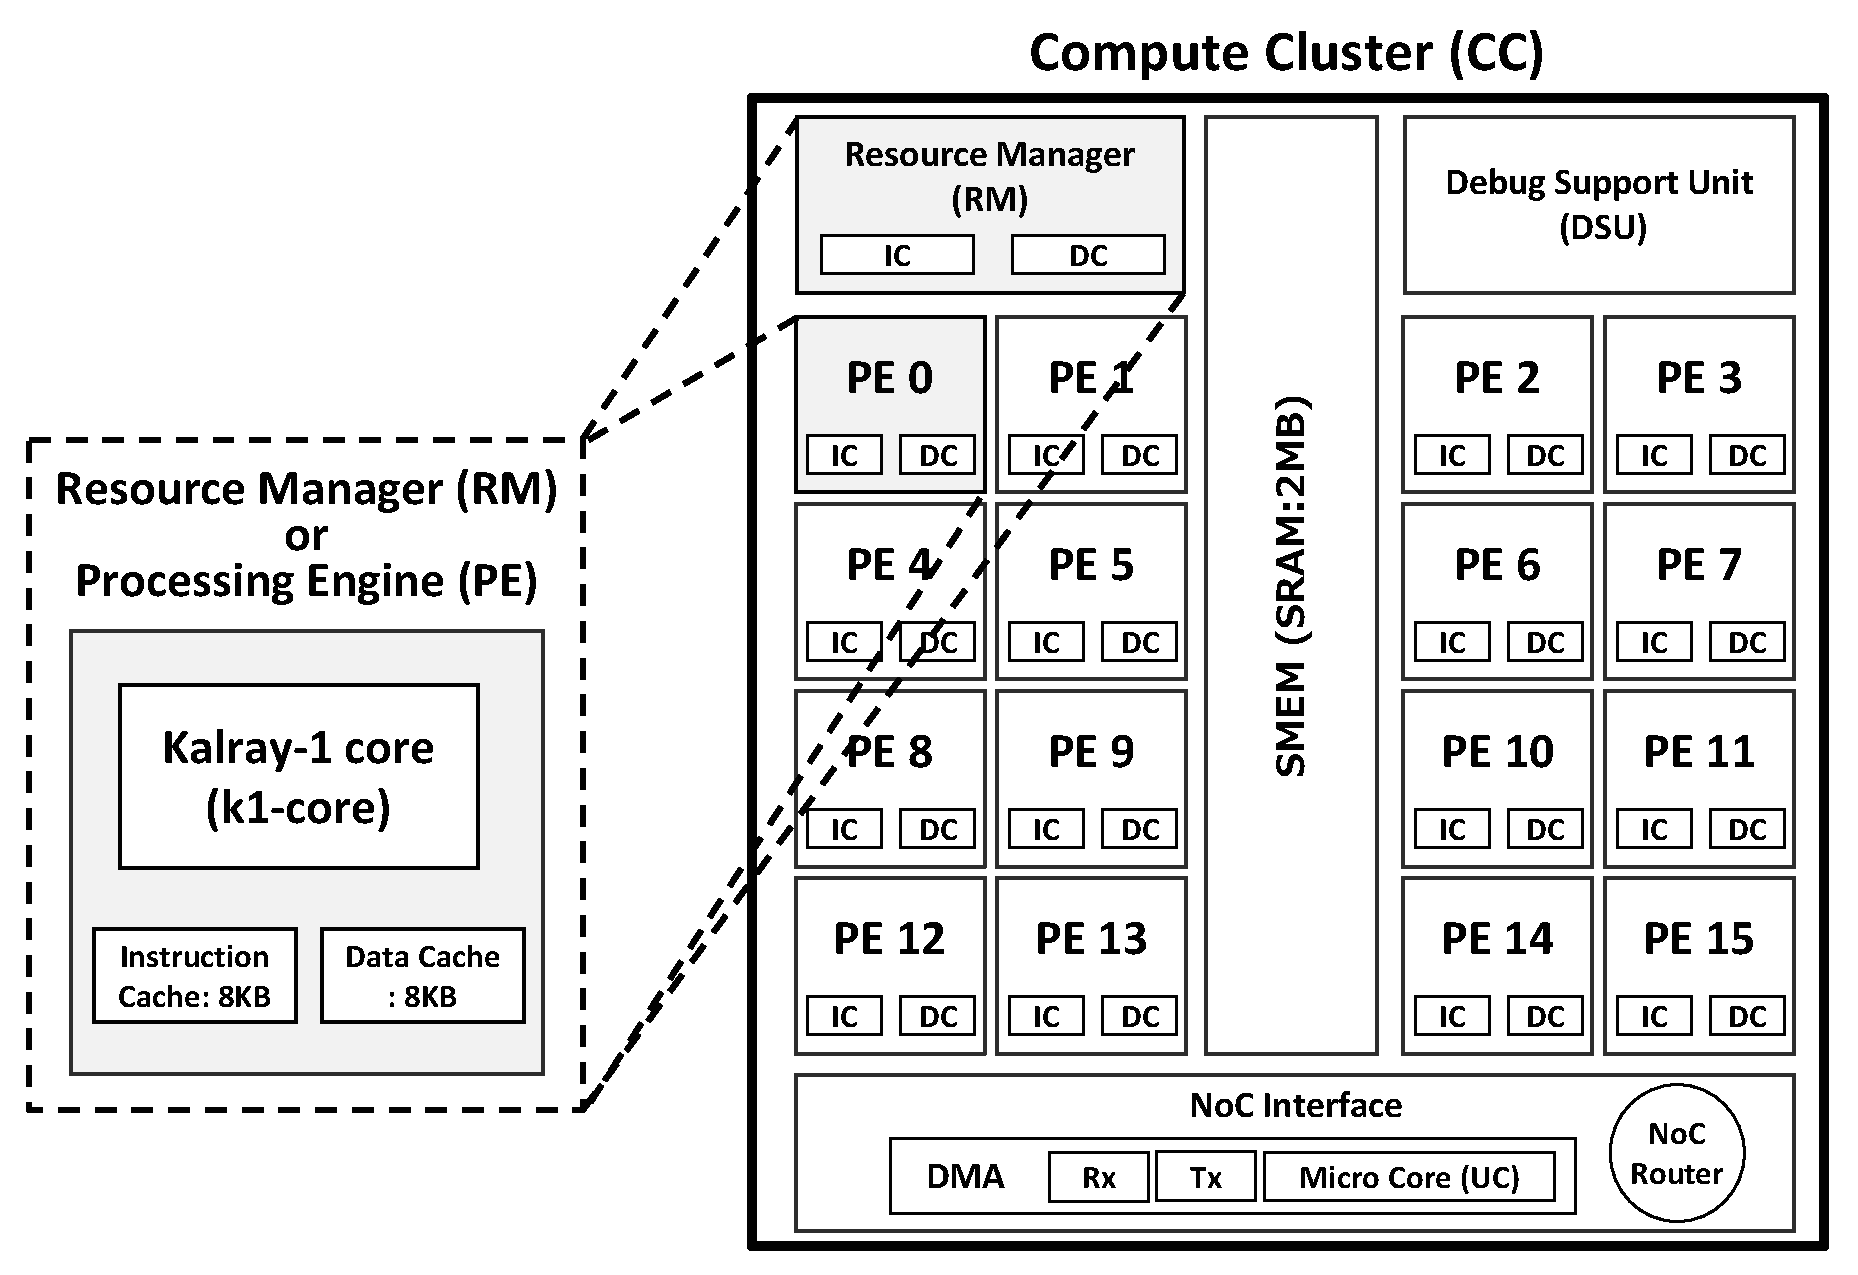
\includegraphics[width=0.7\linewidth]{../figure/cc_architecture.eps}
  \caption{\label{fig:cc_architecture}
    Compute Cluster architecture.}
\end{figure*}

\subsection{Network-on-Chip (NoC)}
\label{sec:noc}
The 16 CCs and the four IOSs are connected by NoC as shown in Fig. \ref{fig:noc_map}.
Furthermore, NoC is constructed \comment{1-12} as the bus network and has routers on each node.

\begin{itemize}
  \setlength{\leftskip}{-5mm}
  \item \textbf{Bus Network}:
  A bus network connects nodes (CCs and IOSs) with torus topology \cite{dally2001route}, which \comment{1-13} involves a low average number of hops when compared to mesh topology \cite{vangal200780}, \cite{taylor2002raw}.
  The network is actually composed of the following two parallel NoCs with bidirectional links (denoted by red lines in Fig. \ref{fig:noc_map}):
  the data NoC (D-NoC) that is optimized for bulk data transfers and the control NoC (C-NoC) that is optimized for small messages at low latency.
  The NoC is implemented with wormhole switching and source routing.
  Data is packaged in variable length packets that are broken into small pieces called flits (flow control digits).
  The NoC traffic is segmented into packets, with each packet including 1-4 header flits and 0-62 payload data flits.
  
  \item \textbf{NoC routers}:
  One node per CC and four nodes per I/O subsystem hold the following two routers of their own: a D-NoC router and a C-NoC router.
  Each RM or IO core on a NoC node is associated with the two aforementioned  NoC routers.
  Furthermore, DMA engines in a NoC interface on the CC/IOS send and receive flits through the D-NoC routers with the Rx interface, the Tx interface, and the UC.
  A mailbox component corresponds to the virtual interface for the C-NoC and enables one-to-one, N-to-one, or one-to-N low-latency synchronization.
  The NoC routers shown in Fig. \ref{fig:cc_architecture} illustrate nodes as R1-16, R128-131, R160-163, R224-227, and R192-195 in Fig. \ref{fig:noc_map}.
  % The NoC routers are illustrated as nodes in Fig. \ref{fig:noc_map}.
  For purposes of simplicity, D-NoC/C-NoC routers are illustrated with a NoC router.
  In both D-NoC and C-NoC, each network node (a CC or an IOS)  includes the following 5-link NoC routers:
  four duplexed links for North/East/West and South neighbors and a duplexed link for local address space attached to the NoC router.
  The NoC routers include FIFOs queuing flits for each direction.
  The data links are four bytes wide in each direction and operate at the CPU clock rates of 600 MHz or 800 MHz, with the result that each tile can transmit/receive a total of 2.4 GB/s or 3.2 GB/s, which is spread across the four directions (i.e., North, South, East, and West).
\end{itemize}  

% \clearpage
\begin{figure}[H]
  \centering
  \includegraphics[width=0.7\linewidth]{../figure/noc_map.eps}
      \caption{\label{fig:noc_map}
    NoC connections (both D-NoC and C-NoC).}
\end{figure}
% \clearpage

\section{Software Model}
\label{sec:software_model}

\begin{figure*}[thbp]
  \centering
  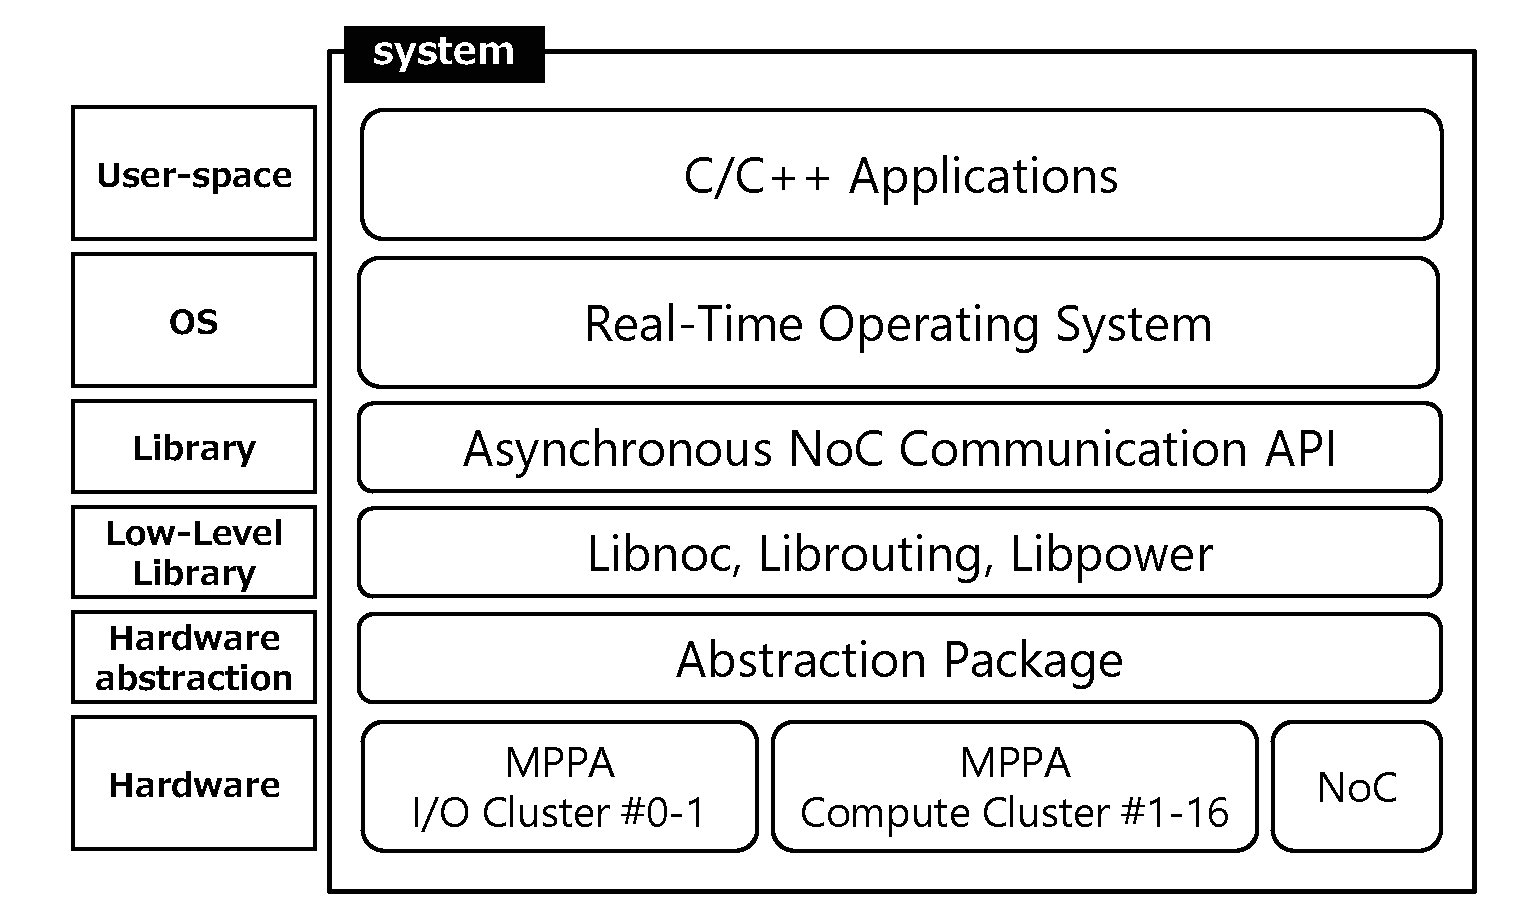
\includegraphics[width=0.7\linewidth]{../figure/softwarestack.eps}   
  \caption{\label{fig:software_stack}
    The software stack of Kalray MPPA-256.}     
\end{figure*}

The software stack used for Kalray MPPA-256 is composed of a hardware abstraction layer, a library layer, an OS, and a user application.  
Fig. \ref{fig:software_stack} shows the software stack used for Kalray MPPA-256 in the present work.
The Kalray system is an extensible and scalable array of computing cores and memory.
With respect to the scalable computing array of the system, it is possible to map several programming models or runtimes such as Linux, a real-time operating system, POSIX API, OpenCL, and OpenMP.
Each layer is described in detail.

In the hardware abstraction layer, an abstraction package abstracts hardware of a CC, an IOS, and NoC.
\comment{1-15} % The abstraction package serves as a system that does not provide any services.
The hardware abstraction is responsible for partitioning hardware resources and controlling access to the resources from the user-space operating system libraries.
\comment{1-16} 
% Additionally, the abstraction package retrieves resources allocated to a partition at any time.
The abstraction sets-up and controls inter-partition communications as a virtual machine abstraction layer.
The hardware abstraction runs on the dedicated RM core.
All the services are provided commonly by an operating system (e.g., virtual memory and schedule) that must be provided by user-space libraries.
% Consequently, each runtime or operating system implements its own services that are optimized to specific needs.
% This is because each programming model or runtime involves different requirements.
A minimal kernel avoids wastage of resources and mismatched needs.

In a low-level library layer, the Kalray system also provides mppa\_noc and mppa\_routing for handling NoC.
Additionally, NoC features such as routing and quality of service are set by the programmer.
mppa\_noc allows direct access to memory mapped registers for their configurations and uses.
This library is designed to cause minimum CPU overhead and also serves as a minimal abstraction for resource allocation.
% Librouting offers a minimal set of functions that can be used to route data between any clusters of the MPPA including unicast (one target) modes or multicast (multiple targets) modes.
mppa\_routing offers a minimal set of functions that can be used to route data between any clusters of the MPPA.
Routing on the network is conducted statically with its own policy.
In addition, mppa\_power enables spawning and waiting for the end of execution of other clusters.

\comment{1-17}
% Routing on the torus network is statically conducted with its own policy.
% The Libpower enables spawning and waiting for the end of execution of a remote cluster.

\subsection{Operating System}
\label{sec:operating_system}
Several operating systems support the abstraction package in the OS layer.
It is difficult for numerous cores such as MPPA to support previous operating systems for single/multicore(s) owing to problems involving parallelism and cache coherency \cite{Wentzlaff2009FOS}, \cite{schupbach2008embracing}.
Here, the following real-time operating systems (RTOSs) supporting MPPA are introduced:

\begin{itemize}
  \setlength{\leftskip}{-5mm}    
  \item \textbf{RTEMS}: Real-Time Executive for Multiprocessor Systems (RTEMS) is a full-featured RTOS prepared for embedded platforms.
  RTEMS supports several APIs and standards, and most notably supports the POSIX API.
  The system provides a rich set of features, and an RTEMS application is mostly a regular C or C++ program that uses the POSIX API.
  \comment{1-18}
  RTEMS runs on the IOC except for the CC.
  
  \item \textbf{NodeOS}: On the CC, the MPPA cluster operating system utilizes a runtime called NodeOS.
  The OS addresses the need for a multicore OS to conform to the maximum possible extent to the standard POSIX API.
  The NodeOS enables a user code by using the POSIX API to run on PEs on the CC.
  First, NodeOS runtime starts on PE0 prior to calling the user main function.
  Subsequently, \texttt{pthread} is called on other PEs.
  
  \item \textbf{eMCOS}: On both CCs and IOSs, eMCOS provides minimal programming interfaces and libraries.
  Specifically, eMCOS is a real-time embedded operating system developed by eSOL (a Japanese supplier for RTOSs) and is the first commercially available many-core RTOS for use in embedded systems.
  The OS implements a distributed microkernel architecture.
  This compact microkernel is equipped with only minimal functions.
  The eMCOS enables applications to operate priority based message passing, local thread scheduling, and thread management on IOSs as well as CCs.
\end{itemize}

RTMES and NodeOS are provided by Kalray and eMCOS is released by eSOL.

\subsection{NoC Data Transfer Methods}
\label{sec:data_transfer_methods}
\comment{TBD: 1-19: To be fully refleshed, Add setup and approach}
This section explains the data transfer methods used in MPPA-256.
For scalability purposes, MPPA-256 implements a clustered architecture that reduces memory contention between numerous cores and associates memory with each cluster.
Sixteen cores are packed in a cluster, and each of these clusters share 2 MB memory (SMEM), as shown in Fig. \ref{fig:cc_architecture}.
This reduces memory contention that frequently occurs with numerous cores and helps to increase the number of cores.
However, the clustered architecture constrains the memory that can be directly accessed by each core.
Communicating with cores outside the cluster requires transferring data between clusters through the D-NoC via NoC interfaces.

In the lowest-level layer, each cluster on MPPA-256 contains hardware for a NoC interface, which has DMA units that handle data receiving and sending: Rx, Tx, and UC interfaces.

An Rx interface is installed on the receiving side to receive data with DMA.
A D-NoC Rx resource must be allocated and configured the Rx to wait for receiving the data.
The DMA in each NoC interface contains 256 D-NoC Rx resources.

The Tx and UC interfaces (explained in Sections \ref{sec:ios} and \ref{sec:cc}) manage the sending side that programs use to send data between clusters.
The UC is a network processor programmed to set threads to send data in DMA.
The UC executes programmed patterns and sends data through the D-NoC without a PE or an RM.
The UC interface results in higher data transfer throughput compared with the direct activation of the Tx interface.
However, the DMA in each NoC interface contains only eight D-NoC UC resources.
Both the interfaces use a DMA engine to access memory and copy data.
Regardless of whether a UC interface is used, a D-NoC Tx resource must be allocated and configured to send data.
In addition, D-NoC UC resources must be allocated and configured, if a UC interface is used.

Several options are available for data transfer between clusters on D-NoC.
Kalray provides mppa\_noc and mppa\_async libraries and eMCOS provides two type of message APIs.
Table \ref{tb:comparison_noc} lists the features of each method for comparison.
The specifications are different for each method; therefore an appropriate method must be chosen according to the application.
For an internal implementations, all methods are based on mppa\_noc which is a low-level NoC communication library that provides interfaces to handle DMA resources, such as Rx, Tx, and UC interfaces for data transfer.
A detailed description of each available NoC data transfer method is given below.

\begin{table*}[thbp]
  \caption{\label{tb:comparison_noc}
    Comparison of NoC Data Transfer Methods}
  \centering
  \scriptsize	                    % text size
  \tabcolsep = 1.5mm              % side-margin in column
  \begin{tabular}{c|ccccccc}
    \hline
    & \multirow{2}{*}{Provider} & \multirow{2}{*}{Model} & Resource & Buffer & DMA & Equality of \\
    & & & Management & Allocation & Type & IOC and CC \\
    \hline
    \hline
    mppa\_noc & Kalray & send/receive & self & user-space & Tx/UC & equal \\
    mppa\_async & Kalray & read/write & auto & user-space & Tx & non-equal\\
    eMCOS message & eSOL & send/receive & auto & kernel-space & Tx & equal \\
    eMCOS session message & eSOL & send/receive & auto & user-space & UC & equal \\
    \hline
  \end{tabular}
\end{table*}

\begin{itemize}
  \setlength{\leftskip}{-5mm}
  \item \textbf{mppa\_noc}: This is the lowest-level NoC communication library for D-NoC and C-NoC components.
  This library handles all interfaces (Rx, Tx, and the UC).
  Users allocate DMA resources and configure them for NoC transport.
  After the data is transferred, users must free the resources.
  Although users must manage DMA resources, the library offers fine-grain control over interfaces, including transport routes on NoC components and send/receive buffers.
  \item \textbf{mppa\_async}: The asynchronous communication API is used for asynchronous operations that involve on one-sided communications between the CC local memory banks and I/O cluster DDR memory. 
  This API is designed to support applications that require remote memory access, whether the DDR memory or the SMEM of other CCs.
  Users must create segments that correspond in whole or in part to the other CC's local memory banks.
  These segments are managed by servers run on the IOC and CC.
  Users initiate an asynchronous write or read process between the local memory and a designated memory segment.
  Two addresses are supplied, one local and one remote from the memory segment.
  \item \textbf{eMCOS message}: eMCOS provides message APIs for communication between threads via Tx interfaces in the D-NoC.
  The destination of a message is a thread, and sending/receiving processes use asynchronous/synchronous modes.
  Users can also configure receiving behavior with masks and priority-based filtering.
  Under the message APIs, data can be exchanged between threads regardless of the cluster on which the thread is running.
  eMCOS runs on IOC and CC to equally manage threads and messages between all clusters.
  Message buffering on each core is managed by eMCOS, and the data sent by DMA through D-NoC are copied to the buffer in eMOCS.
  After resolving the reception order, data are provided by copying non-cache access from the message buffer to user-space addresses.
  \item \textbf{eMCOS session message}: eMCOS provides message APIs for large-data transfer using UC interfaces through D-NoC.
  This API is designed to send large amounts of data rapidly via the UC.
  Users must open sessions which correspond to pairs of send and receive buffers.
  The number of segments is limited by the number of UCs on each cluster.
  Using sessions established in advance, users transport data between clusters.
  The sending/receiving behaviors use asynchronous/synchronous modes.
\end{itemize}


\chapter{Proposed Framework}
\label{chap:proposed_framework}

\begin{figure*}[thbp]
  \centering
  \includegraphics[width=0.9\linewidth]{../figure/roslite/system_model.eps}
  \caption{\label{fig:rosl_system_model}
    Development flow of ROS-lite framework.}
\end{figure*}

The proposed framework, ROS-lite, is a structured communications layer that enables an efficient application development for many-core platforms.
Although the existing ROS is well developed and widely used, it does not support NoC communication on many-core platforms as well as the required features for embedded platforms, such as RTOSs and limited memory.
ROS-lite addresses these challenges and provides a development environment in which ROS nodes run on each core and communicate with each other.
By adapting and extending numerous existing ROS applications, ROS-lite makes porting existing software and new development on embedded platforms much more efficient.
For more information about ROS in general, refer to Appendix A.
As it is based on the existing ROS framework, ROS-lite can communicate with external ROS nodes on another platform.
The tests reported herein used eMCOS as an RTOS and MPPA-256 as an embedded many-core platform.

\section{ROS-lite Toolchain}
\label{sec:toolchain}

\begin{figure*}[thbp]
  \tabcolsep = 0.5mm              % side-margin in column
  \begin{tabular}{cc}
    \begin{minipage}[thbp]{0.59\textwidth}
      \centering
      \includegraphics[width=0.85\linewidth]{../figure/roslite/example.eps}
      \caption{The publish/subscribe model in ROS-lite.}
      \label{fig:rosl_example}
    \end{minipage}
    &
    \begin{minipage}[thbp]{0.39\textwidth}
      \lstinputlisting{../code/roslite_map_two_listenres.map}
      \caption{Map file Description (\texttt{.map}).}
      \label{code:map_file}
    \end{minipage}
  \end{tabular}
\end{figure*}

This section describes ROS-lite in detail.
The development flow for ROS-lite is shown in Fig. \ref{fig:rosl_system_model}.
ROS-lite can run application code written as ROS nodes.
I assume that the applications are written in C++, similar to ROS.
Application developers can adapt source code (application code and message structure files) from existing ROS packages without changing it.
For task mapping, developers edit a map file (\texttt{.map}) and assign ROS nodes to the CCs on many-core platforms.
Developers are required to only edit the map file to modify task mappings.
The ROS nodes as processes on cores are described in terms of a publish/subscribe model, following the message structures defined in message files (\texttt{.msg}).
ROS nodes can communicate with each other via either intra-cluster or inter-cluster routes.
These cores handle intra-cluster communications via shared memory, whereas the inter-cluster are handled via NoC.

ROS-lite toolchain provides a code generation and a build system with a command-line interface to allow an efficient development.
First, as in \textcircled{\scriptsize 1} of Fig. \ref{fig:rosl_system_model}, a template of a map file (\texttt{.map}) is generated from application source code.
The map file (\texttt{.map}) contains node names, the assigned cluster, and the information of topics that are published and subscribed to.
Fig. \ref{code:map_file} can refer for an example of the map file specifications.
These descriptions, except for the assigned cluster number, can be able to be interpreted from ROS nodes to provide code generation for template code.
Application developers can then focus on the number of assigned clusters.
Second, as in \textcircled{\scriptsize 2} of Fig. \ref{fig:rosl_system_model}, header files that defined the message structure are generated from message files (\texttt{.msg}), as in the original ROS.
Note that the generated header files are lighter than when they are in ROS because only the part required by ROS-lite is generated.
This code-generation module is based on the original ROS script, and message files (\texttt{.msg}) can be described as they are in in ROS.
The message files (\texttt{.msg}) do not require any modifications.
Third, in \textcircled{\scriptsize 3} and \textcircled{\scriptsize 4} of Fig. \ref{fig:rosl_system_model}, initialization code for launching processes of ROS nodes are generated from a map file (\texttt{.map}).
ROS nodes are automatically launched as processes scheduled by the RTOS on user-assigned clusters.
Application developers do not have to write code except for the ROS nodes that are used.
Finally, in \textcircled{\scriptsize 5} of Fig. \ref{fig:rosl_system_model}, a build script is generated from the user-defined map file (\texttt{.map}).
The source code of the ROS nodes is built separately for each user-assigned cluster because the executable files are loaded into separate memory banks in each cluster.
This process is conducted by build script.
The build script does not require any modifications when the task mapping is changed by modifying the map file (\texttt{.map}).
The code for the ROS nodes is allocated in a single directory, and each node is automatically built in each user-assigned cluster.

A simple example to understand ROS-lite framework is provided herein.
One node publishes a \emph{chatter} topic and two nodes subscribe to the topic, as shown in Fig. \ref{fig:rosl_example}.
Messages in the \emph{chatter} topic are defined as a string type named \emph{data}.
The publisher node is launched in \emph{cluster 1}, and two subscriber nodes are launched in \emph{cluster 2}, as described by the assigned cluster number in the map file (\texttt{.map}) shown in Fig. \ref{code:map_file}.
Application developers can change the node mapping by modifying of the cluster number field.
Information about topics in the map file (\texttt{.map}) is used to initialize the relation between the topics and the nodes so that ROS-lite directs the process of matching the nodes with topic names.
These fields, for node name and topic information, are generated from source codes of the ROS nodes, and then initialization script for the node relations in ROS-lite are generated from the map file (\texttt{.map}).
Note that the field for the assigned cluster numbers must be filled by application developers.

\section{Design and Implementation}
\label{sec:design_and_implementation}

\begin{figure}[H]
  \centering
  \includegraphics[width=0.8\linewidth]{../figure/roslite/software_stack.eps}
  \caption{\label{fig:rosl_software_stack}
    System stack of ROS-lite on a many-core platform.}
\end{figure}

I tested ROS-lite with an implementation on MPPA-256 as shown in Fig. \ref{fig:rosl_software_stack}.
MPPA-256 is an example of NoC-based clustered many-core processors with distributed memory architecture.
ROS-lite can run on this platform, if memory is limited, as it would be in an embedded application.
ROS-lite allows NoC-based message transfer with low memory consumption.
Note that ROS-lite is a general framework, and other many-core processors can be used with it.

In our test, eMCOS is used as the RTOS for ROS-lite because eMCOS has rich messaging functions, as described in Section \ref{sec:data_transfer_methods}, and can run well on CCs and IOCs.
All threads under ROS-lite are managed by eMCOS.
The light-weight threads so generated are not core-affinity threads.
Threads are not allocated to a specific core within a cluster but are migrated within the specific cluster following the eMCOS scheduling policy.
Internal thread management is thereby improved by eMCOS.

ROS-lite does not have a master server like ROS’s \texttt{ros master}, which helps the original framework to avoid single failures. Nodes in ROS-lite use map files to statically initialize topic information that specifies each node that subscribes to each topic outside its own cluster.
Initialization scripts are generated off-line by the command-line interfaces.
I adopted this off-line initialization process since many specifications about execution time will be fixed ahead of time for most embedded systems.
By eliminating the master server, ROS-lite avoids unnecessary communication between clusters and a single failure point.

I next discuss the internal design of publish/subscribe transport for ROS-lite.
A subscriber's main thread creates a \texttt{message receive function} for each topic, as shown in Fig. \ref{fig:subscriber_design1}.
Subscriber nodes handle message buffering and behavior with one process in ROS-lite.
The design in Fig. \ref{fig:subscriber_design1} can be implemented easily with the message function in eMCOS.
The message function already implements message buffering and NoC transport between threads, but the buffer is allocated in kernel-space and cannot be configured dynamically.
ROS-lite can use mppa\_async and session messaging to address this problem.
ROS-lite adopts mppa\_async because the session message s constrained by the session number by DMA resources.
Session messaging is not a suitable scenario that requires creating many sessions.
Fig. \ref{fig:pubsub_thread_design1} shows the implementation design of publish/subscribe transport in ROS-lite.
Before data transport, the publisher nodes serialize data following the message structure.
ROS-lite's serialization policy is based on the original ROS.
After serialization, the publisher node sends messages to the subscriber nodes listed in topic information, which are initialized by the map file off-line.
Receiving the serialized data size, the subscriber node allocates memory and creates segments for data transport.
Frequent \texttt{alloc} and \texttt{free} of heap memory for each message size conserve the limited memory of the embedded system.
Segments of mppa\_async for transport between clusters are created and destroyed with each transport.
Although this transaction increases overhead, it allows ROS-lite to flexibly handle variable-length messages, such as vectors.

To prevent the simultaneous execution of callback functions and design ensure that each node only runs as one process, it is necessary to use the design shown in Fig. \ref{fig:subscriber_design2}, not the design of Fig. \ref{fig:subscriber_design1}.
A callback queue manages the order of callback functions to be executed at the subscriber node.
This queue can be implemented simply with eMCOS message buffering.
eMCOS messaging is suitable for small-size data transport, and the data pushed for the queue is small because it only contains pointers to the callback function and received messages.
Fig. \ref{fig:pubsub_thread_design2} shows an example of ways in which the design in Fig. \ref{fig:subscriber_design2} can be implemented.

ROS-lite supports original ROS source code to enhance porting and development efficiency for applications running on many-core processors.
ROS-lite provides the same interfaces as the ROS API for application developers who are not familiar with NoC interfaces.
Figs. \ref{code:talker}, \ref{code:listener}, and \ref{code:msg} provide source code for the scenario in Fig. \ref{fig:rosl_example}.

\clearpage
\vspace{-10mm}

\begin{figure*}[thbp]
  \centering
  \includegraphics[width=0.9\linewidth]{../figure/roslite/design/subscriber_design1.eps}
  \vspace{-10mm}
  \caption{\label{fig:subscriber_design1}
    Structure of subscriber node.}
  \vspace{-10mm}
\end{figure*}

\begin{figure*}[thbp]
  \centering
  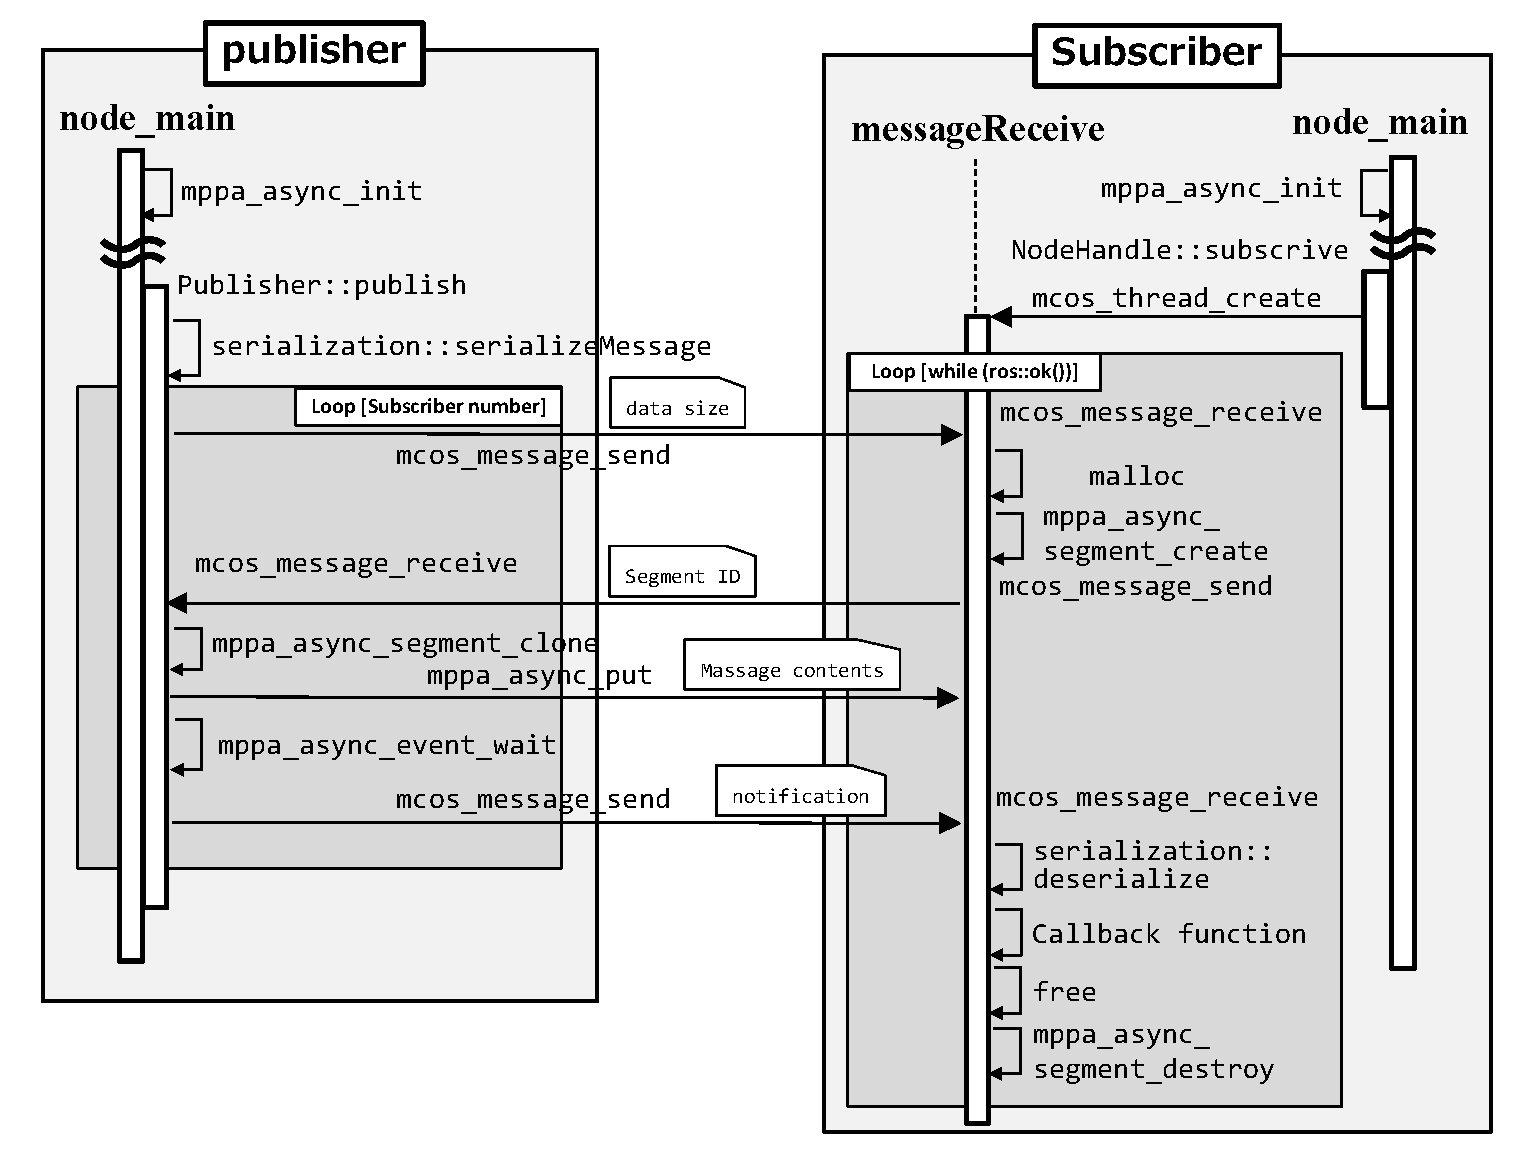
\includegraphics[width=0.9\linewidth]{../figure/roslite/design/pubsub_thread_design1.eps}
  \caption{\label{fig:pubsub_thread_design1}
    Design of publish/subscribe sequence of Fig. \ref{fig:subscriber_design1} without message buffering.}
    \vspace{-10mm}
\end{figure*}

\vspace{-10mm}

\begin{figure*}[thbp]
  \centering
  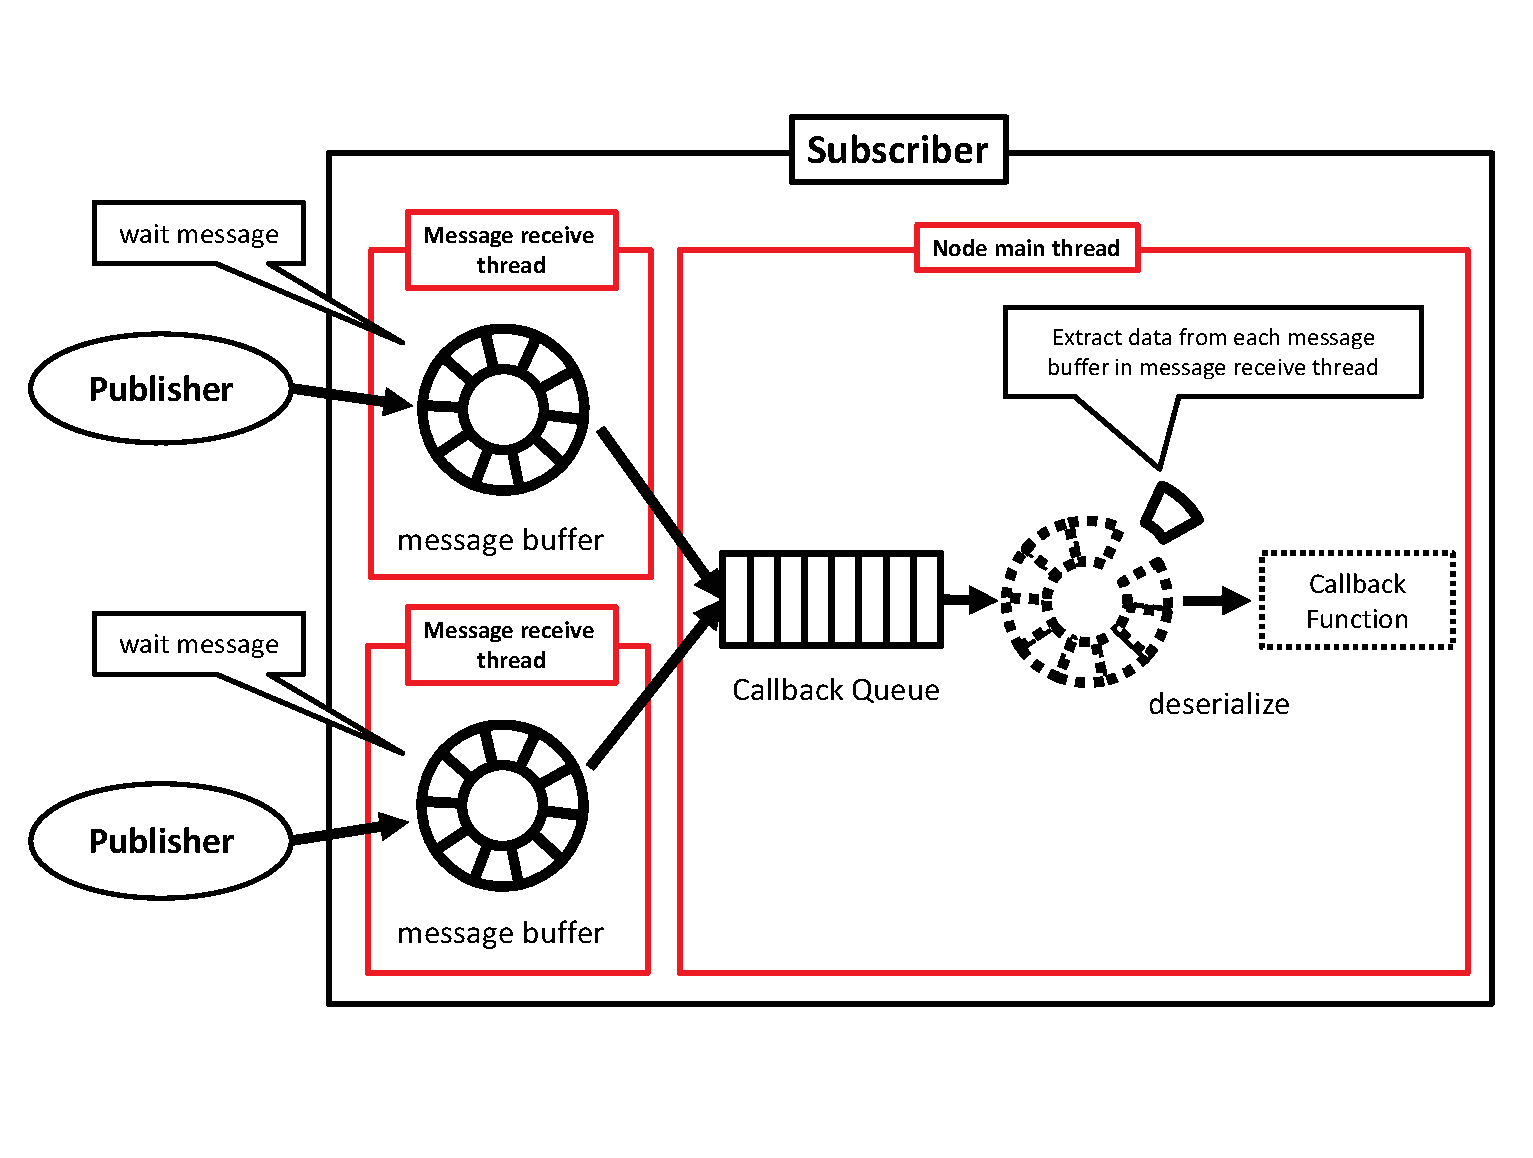
\includegraphics[width=0.9\linewidth]{../figure/roslite/design/subscriber_design2.eps}
  \vspace{-10mm}
  \caption{\label{fig:subscriber_design2}
    Structure of subscriber node with callback queue.}
    \vspace{-10mm}
\end{figure*}

\begin{figure*}[thbp]
  \centering
  \includegraphics[width=0.9\linewidth]{../figure/roslite/design/pubsub_thread_design2.eps}
  \caption{\label{fig:pubsub_thread_design2}
    Design of publish/subscribe sequence of Fig. \ref{fig:subscriber_design2}.}
  \vspace{-10mm}
\end{figure*}

\begin{figure*}[thbp]
  \centering
  \lstinputlisting{../code/talker.cpp}
  \caption{\label{code:talker}
    An example of a C++ source code (\texttt{.cpp}): a publisher node.}
\end{figure*}

\begin{figure*}[thbp]
  \centering
  \lstinputlisting{../code/listener.cpp}
  \caption{\label{code:listener}
    An example of a C++ source code (\texttt{.cpp}): a subscribe node.}
\end{figure*}

\begin{figure*}[thbp]
  \centering
  \lstinputlisting{../code/String.msg}
  \caption{\label{code:msg}
    An example of a message file (\texttt{.msg}): string message type.}
\end{figure*}

\chapter{Evaluations}
\label{chap:evaluations}
First, this chapter involves examining two types of evaluations: a D-NoC data transfer evaluation in which latency characteristics of interfaces and memory type are explored and a matrix calculation evaluation that demonstrates the parallelization potential of the MPPA-256 and its memory access characteristics.
Subsequently, I conduct a practical self-driving application to examine the practicality of NUMA many cores.
% Finally, we arrange lessons learned from above evaluations.
The following evaluations are all conducted on real hardware boards with eMCOS.

\section{D-NoC Data Transfer}
\label{sec:dnoc_eval}

\subsection{Situations and Assumptions}
\label{sec:situations_and_assumptions2}

\begin{figure}[thbp]
  \centering
  \includegraphics[width=0.5\linewidth]{../figure/noc_routes_old.eps}
      \caption{\label{fig:noc_routes}
    Four D-NoC routes used in the evaluation.}
\end{figure}

This evaluation involves clarifying end-to-end latency by considering the relation among interfaces (Tx or UC), routing on NoC, and memory type (DDR or SMEM).
This is achieved by preparing four routes as shown in Fig. \ref{fig:noc_routes}.
The routes on the D-NoC map (Fig. \ref{fig:noc_map}) contain various connections between routers, a direct link, a cross-link, and a flying link.
With respect to the case of routes from the IOS routers to the CC routers, transmitted data are allocated in the DDR or IO SMEM.
The CC includes only the SMEM as shown in Fig. \ref{fig:cc_architecture}.
% A low-level library is directly used to transfer data with D-NoC.
The transferred data correspond to 100 B, 1 KB, 10 KB, 100 KB, and 1 MB.
The buffers are sequentially allocated in DDR or SRAM (IO SMEM or CC SMEM).
The capacity of the CC SMEM is 2 MB, and thus it is assumed that the appropriate communication buffer size is 1 MB.
Given this assumption, the other memory area corresponds to the application, libraries, and an operating system.
End-to-end latencies are measured 1,000 times in numerous situations as shown in Figs. \ref{fig:DDR_tx}, \ref{fig:DDR_uc}, and \ref{fig:IO_SMEM_tx}, and boxplots are obtained, as depicted in Figs. \ref{fig:IO_SMEM_uc}, \ref{fig:tx_uc_log}, and \ref{fig:tx_uc}.
In the evaluation setting, I minimize traffic conflicts to focus on the relation between end-to-end latency and routing on NoC.

\subsection{Influences of Routing and Memory Type}
\label{sec:routing_and_memory}

\comment{1-20, 1-21}
Data transfer latencies between an IOS and a CC are influenced little by routing.
This involves preparing two interfaces (Tx and UC), three routes (direct link, cross-link, and detour route), and two memory locations in which the transferred data are allocated.
As shown in Figs. \ref{fig:DDR_tx}, \ref{fig:DDR_uc}, \ref{fig:IO_SMEM_tx}, and \ref{fig:IO_SMEM_uc}, 
end-to-end latency scales exhibit a linear relation with data size, and there are no significant differences between the three routes with respect to data transfer latency.
This result is important in a torus topology NoC because the number of minimum steps exceeds that in a mesh topology. 
It is observed that queuing in NoC routers and hardware distance on a NoC are not dominant factors for latency.
The router latency, the time taken in transmitting and receiving transactions in an RM, exceeds those of other transactions.
Additionally, it is briefly recognized that the speed of the UC exceeds that of the Tx.
The data are arranged as shown in Figs. \ref{fig:tx_uc_log} and \ref{fig:tx_uc} to facilitate a precise analysis with respect to the interface and memory location.
In those figures, only the cross-link from the IOS to CC5 is accepted because routes do not influence latency.
To facilitate intuitive recognition, two kinds of figures are arranged: a logarithmic and a linear axis.

In the Tx interface, DDR causes a large increase in latency.
The time taken by the DDR is twice that of the IO SMEM as shown in Fig. \ref{fig:tx_uc_log}.
This is due to the memory access speed characteristics of DRAM and SRAM.
In the Tx interface, it is necessary for an IO core on an IOS to operate the DMA in the IOS NoC interface.
This is attributed to the fact that the core is involved in processing.
The speed of the data transfer latency between CCs exceeds that between an IOS and a CC.
This result indicates that the MPPA-256 is optimized for communication between the CCs.

With respect to the UC interface, the latency is not significantly affected by the location at which the transferred buffer is allocated (i.e., DDR or SMEM).
Similar latency characteristics are observed in Fig. \ref{fig:tx_uc_log}.
In the case of the UC interface, an IO core on the IOS does not involve a DMA transaction.
A UC in the NoC interface executes a programmed thread sending data.
This evaluation result suggests that the slow access speed of the DDR is not significant in the case of the UC.
In a manner similar to that of the Tx interface, the speed of the data transfer latency between CCs exceeds that between an IOS and a CC.

% \clearpage

\begin{figure*}[thbp]
  \tabcolsep = 0.5mm              % side-margin in column
  \begin{tabular}{cc}
    % \setcounter{figure*}{9}
    \begin{minipage}[thbp]{0.49\textwidth}
      \includegraphics[width=1.0\linewidth]{../../R/mppa/graph/eps/BoxPlot_DDR_tx.eps}
      \caption{Data transfer with Tx from IO DDR to CC.}
      \label{fig:DDR_tx}
    \end{minipage}
    &
    % \setcounter{figure*}{11}
    \begin{minipage}[thbp]{0.49\textwidth}
      \includegraphics[width=1.0\linewidth]{../../R/mppa/graph/eps/BoxPlot_DDR_uc.eps}
      \caption{Data transfer with UC from IO DDR to CC.}
      \label{fig:DDR_uc}
    \end{minipage}
  \end{tabular}
\end{figure*}

\begin{figure*}[thbp]
  \tabcolsep = 0.5mm              % side-margin in column
  \begin{tabular}{cc}
    % \setcounter{figure*}{9}
    \begin{minipage}[thbp]{0.49\textwidth}
      \includegraphics[width=1.0\linewidth]{../../R/mppa/graph/eps/BoxPlot_IO_SMEM_uc.eps}
      \caption{Data transfer with UC from IO SMEM to CC.}
      \label{fig:IO_SMEM_tx}
    \end{minipage}
    &
    % \setcounter{figure*}{11}
    \begin{minipage}[thbp]{0.49\textwidth}
      \includegraphics[width=1.0\linewidth]{../../R/mppa/graph/eps/BoxPlot_IO_SMEM_uc.eps}
      \caption{Data transfer with UC from IO SMEM to CC.}
      \label{fig:IO_SMEM_uc}
    \end{minipage}
  \end{tabular}
\end{figure*}

\begin{figure*}[thbp]
  \tabcolsep = 0.5mm              % side-margin in column
  \begin{tabular}{cc}
    % \setcounter{figure*}{9}
    \begin{minipage}[thbp]{0.49\textwidth}
      \includegraphics[width=1.0\linewidth]{../../R/mppa/graph/eps/BoxPlot_Tx_vs_UC_log.eps}
      \caption{Data transfer with Tx/UC (logarithmic axis).}
      \label{fig:tx_uc_log}
    \end{minipage}
    &
    % \setcounter{figure*}{11}
    \begin{minipage}[thbp]{0.49\textwidth}
      \includegraphics[width=1.0\linewidth]{../../R/mppa/graph/eps/BoxPlot_Tx_vs_UC.eps}
      \caption{Data transfer with Tx/UC (linear axis).}
      \label{fig:tx_uc}
    \end{minipage}
  \end{tabular}
\end{figure*}

\clearpage

\section{Matrix Calculation}
\label{sec:martix_eval}

\subsection{Situations and Assumptions}
\label{sec:situations_and_assumptions1}

\begin{figure}[H]
  \centering
  \includegraphics[width=0.5\linewidth]{../figure/matrix_calculation.eps}
  \caption{\label{fig:mat_calc}
    Matrix calculation situations.}
\end{figure}

In the evaluation, the matrix calculation time and parallelization potential of MPPA-256 are clarified.
Matrix calculations are conducted in an IOS and CCs.
Three computing situations are considered as shown in Fig. \ref{fig:mat_calc}.
The first situation involves computing in the IOS where four cores are available.
To analyze memory access characteristics, a matrix buffer is allocated in the IO DDR and SMEM.
The second situation involves computing in a CC in which 16 cores are available.
The third situation involves offload-computing using an IOS and four CCs.
Parallelized processing is executed with four CCs and SMEMs.
A few cores in the IOS and CC manage the parallelized transaction.
The method can handle large amount of data in which one cluster is not sufficient, because buffer capacity is not limited to 2 MB in the SMEM.
Parallelized processing and the total capacity of the SMEM are superior to single IOS or CC computations. 
With respect to the IOS, the application can handle large capacity data only in the DDR.
However, in this method, distributed memories are used to deal with large capacity data in the SMEM.
Thus, it is necessary for IOS and CC cores to access matrix buffers without cache to avoid cache coherency difficulties.
To facilitate faster data transfer, a portion of the matrix buffer is transmitted in parallel as shown in Fig. \ref{fig:mat_calc}.

Matrix calculation time is analyzed with parallelization and memory allocation.
Additionally, the influences of a cache are analyzed because cache coherency is an important issue in many-core systems.
There are several cases in which applications must access specific memory space without a cache because MPPA does not guarantee cache coherency between PEs.
With respect to the given assumptions, the maximum total buffer size is 1 MB, and thus three matrix buffers are prepared, each of size 314 KB.
Matrix A and Matrix B are multiplied, and the result is stored in Matrix C.
The total for the three matrices is set as approximately 1 MB.
I assume that the remainder of the SMEM (1 MB) is occupied with system software and applications in the CC.

\subsection{Influences of Cache and Memory Type}
\label{sec:cache_and_memory}
First, matrix calculation time with the cache in the IOS and CC is depicted in Fig. \ref{fig:mat_calc_cache}.
There are almost no differences between the IO DDR, IO SMEM, and CC SMEM due to the cache.
A 128 KB data cache in the IOS works well and compensates for the DDR delay.
Additionally, it is observed that calculation time scales exhibit a linear relation with the number of threads.
This corresponds to ideal behavior with respect to parallelization.

Second, matrix calculation time without a cache in the IOS and CC is shown in Fig. \ref{fig:mat_calc_uncache}.
The absence of a cache, results in a fourfold increase in the DDR and a large difference arises with respect to the SMEM.
Another notable result is that calculation speed in the CC SMEM exceeds that of the IO SMEM.
This characteristic is hidden in the calculation with the cache.
The computing cores physically involve the same cores in the IOS and CC, and thus it is considered that the characteristics and physical arrangement of the SMEM exert a significant effect.
This is an interesting result since there is a large difference that cannot be ignored.
It is also observed that calculation time exhibits a linear relation with the number of threads.
Furthermore, in the CC SMEM, the calculation speed without the cache exceeds that with cache.
This result is contrary to intuition, and a cache line problem is conceivable.
When a small data cache (8 KB) in a PE of the CC does not function adequately and an application always misses the cache, memory access will pay the time for a noncached data access and the cost to refill the cache line.
As a result, the memory access speed without the cache exceeds that with it.

\clearpage

\begin{figure*}[thbp]
  \centering
  \includegraphics[width=.9\linewidth]{../figure/BarGraph_matrix_with_cache.eps}
  \caption{Matrix calculations in IOS and CC with cache.}
  \label{fig:mat_calc_cache}
\end{figure*}

\begin{figure*}[thbp]
  \centering
  \includegraphics[width=.9\linewidth]{../figure/BarGraph_matrix_without_cache.eps}
  \caption{Matrix calculations in IOS and CC without cache.}
  \label{fig:mat_calc_uncache}
\end{figure*}

\subsection{Four CCs' Parallelization}
\label{sec:four_CCs}
Finally, matrix calculation with offload-computing in an IOS and CCs is shown in Figs. \ref{fig:mat_calc_offload_314} and \ref{fig:mat_calc_offload_640}.
In this case, it is assumed with respect to the calculation of large matrices that the total capacity exceeds 1 MB.
The offloading result is compared with the IO DDR (cached) owing to the aforementioned assumption.
The aggregate calculation is obtained by offloading on the four CCs to perform a multiplication of a tile of Mat A and a tile of the transpose of Mat B.
This produces an overhead irrespective of the number of threads as shown in Figs. \ref{fig:mat_calc_offload_314} and \ref{fig:mat_calc_offload_640}.

However, the speed involved in offloading the result exceeds that of the IO DDR (cached).
The result indicates several important facts.
First, D-NoC data transfer produces little overhead latency.
Second, the speed of DMA memory access to DDR exceeds that of the IO core's memory access, even if target memory is allocated on the DDR.
In the offloading case, a DMA accesses matrix buffers on the DDR and transfers the buffers from the IO DDR to each CC SMEM.
Subsequently, PEs in the CC access matrix buffer the calculation without a cache.
The overhead of data transfer and DMA memory access is small, and thus parallel data transmission and distributed memory are practical in the case of MPPA-256.
The impact of offloading increases when the matrix is large as shown in Fig. \ref{fig:mat_calc_offload_640}.
Only a portion of the matrix is allocated in CCs, and thus it is possible to handle larger matrix buffers.

Additionally, 640 KB matrices are prepared, and matrix calculation is evaluated with offload-computing.
The speed of the offloading result exceeds that of the IO DDR result with respect to the 314 KB matrices in Fig. \ref{fig:mat_calc_offload_314}.
In these offloading evaluations, each CC concurrently transmits calculation results to the IOS.
\comment{1-22}
When Matrix C in which calculation results are stored is allocated in the DDR, the NoC router's FIFOs sometimes overflow and cause an error due to memory access delay of the DDR.
The transmission protocol would ideally be expected to prevent this error, and flow control is intended as future work for MPPA-256.
Currently, to avoid this error, Matrix C must be allocated in the IO SMEM.
Note that the above evaluation results when Matrix C is allocated in the DDR.


\begin{figure*}[thbp]
  \tabcolsep = 0.5mm              % side-margin in column
  \begin{tabular}{cc}
    \begin{minipage}[thbp]{0.49\textwidth}
      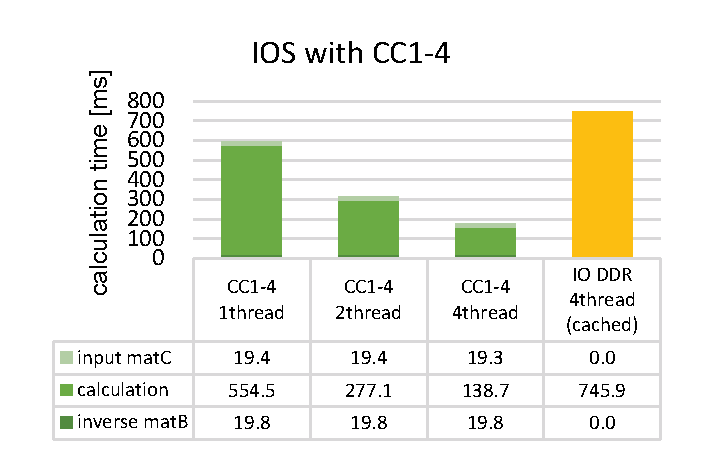
\includegraphics[width=0.9\linewidth]{../figure/BarGraph_matrix_with_CCs_314.eps}
      \caption{Matrix calculations with offload computing (314 KB matrix x 3).}
      \label{fig:mat_calc_offload_314}
    \end{minipage}   
    &
    % \setcounter{figure*}{11}
    \begin{minipage}[thbp]{0.49\textwidth}
      \includegraphics[width=0.9\linewidth]{../figure/BarGraph_matrix_with_CCs_640.eps}
      \caption{Matrix calculations with offload computing (640 KB matrix x 3).}
      \label{fig:mat_calc_offload_640}
    \end{minipage}
  \end{tabular}
\end{figure*}

\section{Practical Application}
\label{sec:practical_application}
This work adopts a portion of a self-driving system and this section demonstrates the parallelization potential of the MPPA-256.
I selected an algorithm for vehicle self-localization written in C++ in Autoware, open-source software for urban self-driving \cite{autoware}, and a parallelized part of it.
(Please refer to Appendix B: Autoware.)
The self-localization adopts the normal-distribution transform matching algorithm \cite{magnusson2009three} implemented in the Point Cloud Library \cite{pcl}.
A diagram depicting self-localization is shown in Fig. \ref{fig:ndt_matching_situation}.

% The self-localization algorithm is primarily divided into two processes: \emph{RadiusSearch} which searches for several nearest neighbor points for each query and calculates the distance, and \emph{Derivatives} which calculates the derivative to determine the convergence of the matching operation.
% As shown in Fig. \ref{fig:ndt_matching_situation}, 
% This evaluation parallelized \emph{Derivatives} onto 16 CCs and the remainder of the algorithm was executed on the IOS with its four cores.
% To parallelize \emph{RadiusSearch}, the algorithm of the nearest neighbor search needs to be redesigned because the data to be searched exceeds 1 MB.
% Redesigning this algorithm will be part of a future work.

The self-localization algorithm is composed primarily of the \emph{computeTransform} function which searches for several nearest neighbor points for each scan query and calculates a matching transformation.
This evaluation parallelized a part of \emph{computeTransform} onto 16 CCs and the remainder of the algorithm was executed in parallel on the IOS with its four cores.
To parallelize the remainder of \emph{computeTransform} in CCs, the algorithm of the nearest neighbor search must be redesigned because the data to be searched exceeds 1 MB.
Redesigning this algorithm is reserved for future work, and there is room for improvement through the parallelization potential of the MPPA-256.

As shown in Fig. \ref{fig:ndt_matching}, the evaluation of the parallelized self-localization algorithm indicates the average execution time for each convergence and demonstrates that the parallelization accelerates the \emph{computeTransform} process.
% Because the reduction of the execution time of \emph{computeTransform} involves reducing the number of loops for convergence, the execution times of \emph{RadiusSearch} and other parts are also shortened.
The query can be assumed to be 10 Hz in many automated driving systems.
Thus, this tuning successfully meets the deadline.
This parallelized algorithm was executed on simulated and real car experiments in our test course and worked successfully.
The steering, accelerator, and brake are automatically controlled based on the results of MPPA-256.
A demonstration video of the adaptation of the parallelized self-localization algorithm to Autoware on eMCOS can be seen at: https://youtu.be/wZyqF90c5b8  

\begin{figure*}[thbp]
  \tabcolsep = 0.5mm              % side-margin in column
  \begin{tabular}{cc}
    \begin{minipage}[thbp]{0.49\textwidth}
      \centering
      \includegraphics[width=1.0\linewidth]{../figure/ndt_matching.eps}
      \caption{\label{fig:ndt_matching_situation}
      A situation of vehicle self-localization execution.}
    \end{minipage}   
    &
    % \setcounter{figure*}{11}
    \begin{minipage}[thbp]{0.49\textwidth}
      \includegraphics[width=1.0\linewidth]{../figure/BarGraph_ndt_matching.eps}
      \caption{\label{fig:ndt_matching}
      Vehicle self-localization of the partially parallelized self-driving application.}
    \end{minipage}
  \end{tabular}
\end{figure*}


\section{Lessons Learned}
\label{sec:lessons}
\comment{TBD: 3-4}
Thus far, in Chapter \ref{chap:evaluations}, I have quantitatively clarified the characteristic of data transfer and parallel computing on NoC-based embedded many-core platforms.
I can obtain insight and guidelines for users and developers of NoC-based embedded many-core platforms through MPPA-256.

From evaluations of D-NoC data transfer, you can learn two lessons: the influences of NoC routing and DMA.
First, data transfer latencies between clusters are hardly influenced by routing for users as shown in Figs. \ref{fig:DDR_tx}, \ref{fig:DDR_uc}, \ref{fig:IO_SMEM_tx}, and \ref{fig:IO_SMEM_uc}.
Software transactions of transmitting and receiving in routers and RM are dominant factors for latencies.
This is understandable owing to the minimized traffic conflicts of the evaluation setting.
However, when the influence of routing comes to intensive concurrent traffic over a large portion of the network, different routes might still have nontrivial impacts on the end-to-end data transfer delay, especially for a detour route of a longer length.
Second, in the IOS, the latency of a UC is not significantly affected by the memory location, the DDR or SMEM, at which the transferred buffer is allocated from the evaluation of Fig. \ref{fig:tx_uc_log}.
The merit of the UC is profitable for users because this is a common situation for transferring data from the DDR to the CC SMEM using the UC, especially for large amount of data.

From microbenchmarks of matrix calculation, you can learn three lessons of memory access: characteristics of the SMEM, influences of a cache, and data flow control on D-NoC.
First, the memory access speed of the CC SMEM exceeds that of the IO SMEM as shown in Fig. \ref{fig:mat_calc_uncache}.
There is a significant difference, which is a major reason to work actively in the CC.
Second, I indicate quantitatively that the calculation speed without the cache in the CC SMEM in Fig. \ref{fig:mat_calc_uncache} exceeds that with the cache in Fig. \ref{fig:mat_calc_cache}.
It is generally known that there is cache overhead when a miss hit occurs frequently, but it is notable that there is a substantial difference that cannot be ignored by the influences of a cache line.
Third, when data are transferred in parallel from multiple CCs to the IO DDR, NoC routers' FIFO sometimes overflows owing to memory access delays of the DDR.
This would ideally be expected to be prevented by the transmission protocol and flow control.

From the practical application viewpoint, since I parallelize the vehicle self-localization algorithm of the self-driving system, NoC-based embedded many-core systems can be used practically in real environments.
I applied for parallel data transfer from an IOS to CCs and parallel computing on the IOS and CCs by using the CC SMEM as scratch pad memory.    
I also conducted demonstration experiments with real environments and confirmed the practicality of NoC-based embedded many-core systems.

\chapter{Related Work}
\label{chap:related_work}
\memo{Add comparison to eMCOS, Facrored OS, and Barrelfish}
\memo{Add ROS-lite comparison table and descriptions}
This chapter compares many-core platforms and discusses previous work related to multi-/many-core platforms.
First, comparison of many-core platforms to other platforms is discussed.
Second, the Kalray MPPA-256 which this work focuses on is compared to other COTS multi-/many-core components, and I summarize the features of MPPA-256.
Finally, discussions of previous work and comparisons with them are described.

% Recently, studies indicate that the single core processors are characterized by limited computation performance.
% Pollack stated that a single core is inefficient \cite{pollack1999new} and that Moore's law \cite{moore2006cramming} is no longer applicable.
% Therefore, extant CPUs are not sufficient to satisfy increasing computation demands.
% The shift from a single core in real-Time and embedded systems has occurred \cite{saidi2015shift}. 
% Many other platforms including many-core are developed and researched by current studies.

Table \ref{tb:comparison_platforms} summarizes the features of many-core platforms with those of other platforms.
For instance, the GPU is a powerful device to enhance computing performance and has great potential in specific areas (for e.g., image processing, and learning).
\comment{1-24}
However, the GPU is mainly used for a specific purpose and its predictability is not suitable for real-time systems.
It is difficult to use a GPU for many kinds of applications and to guarantee its reliability due to the GPU architecture.
Many-core processors based on CPU are significantly superior to GPU with respect to software programmability and timing predictability.
\comment{1-25}
Additionally, it is commonly known that many-core platforms such as MPPA-256 involve a reasonable power consumption \cite{kanter2015kalray}.
In contrast, the GPU consumes a significant amount of power and generates considerable heat.
This is a critical problem for embedded systems.
FPGAs are also high-performance devices when compared to CPUs.
They are efficient in terms of power consumption.
FPGAs guarantee predictability and efficient processing.
% They are suitable for time-critical computing \cite{de2015kalray}.
\comment{1-26}
% However, DSPs cannot be used for many kinds of applications and programming.
However, FPGAs are difficult for software developers and are not a substitute for CPU since their software model is significantly different from that of CPU.
Many-core platforms can potentially replace single/multi core CPU as they possess ease of programming and scalability.

Based on the aforementioned background, many COTS multi-/many-core components are developed and released by several vendors.
(e.g., MPPA-256 by Kalray, \cite{de2014time}, Tile-Gx by Tilera \cite{ramey2011tile}, \cite{schooler2010tile}, Tile64 by Tilera \cite{bell2008tile64}, and Xeon Phi by Intel \cite{chrysos2014intel}, \cite{chrysos2012intel}, Single-chip Cloud Computer (SCC) by Intel \cite{baron2010single}).
The present work focuses on the Kalray MPPA-256, which is designed for embedded applications.
Kalray \cite{de2014time} presented clustered many-core architectures on the NoC that pack 256 general-purpose cores with high energy efficiency.


\comment{1-27}
MPPA-256 is superior to other COTS multi-/many-core components in terms of the scalability of the number of cores and the power efficiency, as shown in Table \ref{tb:comparison_manycore}.
\comment{1-28}
In terms of scalability, MPPA-256 uses 256 cores, whereas other COTS multi-/many-core components have 64 cores or the number of cores around it.
This scalability of cores is attributed to the NUMA memory architecture; each cluster of 16 cores contains its own local shared memory.
The precise hardware model is described in Section \ref{sec:hardware_model}.
When all cores share the global DDR memory as in other platforms excluding MPPA-256, specific bus/network routes receive extremely large loads and memory access contention frequently occurs.
Local shared memory reduces the above problems and helps the scalability of the number of cores.
% This is why MPPA-256 has succeeded in scaling up to 256 cores and what the ``scalability'' column of Table \ref{tb:comparison_manycore} means.
However, the NUMA memory architecture restricts the capacity of the memory and requires a data copy from the DDR with NoC.
This restriction makes the use of existing applications difficult especially in the case of applications that require more memory.
As a result, owing to the NUMA memory architecture, the portability of code porting to MPPA-256 is inferior to that of other COTS platforms, as shown in Table \ref{tb:comparison_manycore}.

In terms of power efficiency, MPPA-256 realizes superior energy efficiency despite its large number of cores \cite{kanter2015kalray}.
The total clock frequency per watt is the highest of the current COTS multi-/many-core components.
The power consumption of the MPPA processor ranges between 16 W at 600 MHz and 24 W at 800 MHz.
% While MPPA-256 and TILE64 \cite{bell2008tile64} target the embedded systems, other COTS components consider the HPC accelerator.
% Their clock frequency per core exceeds that of embedded solutions.
You must distinguish the COTS multi-/many-core components according to their requirements with reference to Table \ref{tb:comparison_manycore}.
MPPA-256 is typically accepted with respect to many-core platforms and the model has been used in previous work \cite{becker2016contention}, \cite{carle2014static}, \cite{perret2016mapping}, \cite{perret2016predictable}.

Previous work has examined real-time applications on many-core platforms, including MPPA-256.
Multiple opportunities and challenges of multi-/many-core platforms are discussed in \cite{saidi2015shift}.
The shift to multi-/many-core platforms in real-time and embedded systems is also described. 

Based on the above background, several task mapping algorithms for multi/many-core systems have been proposed \cite{carle2014static}, \cite{faragardi2014communication}, \cite{perret2016mapping}.
Airbus \cite{perret2016mapping} proposes a method of directed acyclic graph (DAG) scheduling for hard real-time applications using MPPA-256.
In \cite{faragardi2014communication}, a mapping framework is proposed on the basis of AUTOSAR which is applied as a standard architecture to develop automotive embedded software systems \cite{furst2009autosar}.
AUTOSAR task scheduling considering contention in shared resources is presented in \cite{becker2016contention}.

By examining the above mapping algorithms of real-time applications, previous work \cite{deDinechin2014GSN}, \cite{denet2017work}, \cite{kanter2015kalray}, \cite{perret2016predictable} has analyzed the potential of MPPA-256 and data transfer with NoC, as shown in Table \ref{tb:comparison_relatedwork}.
MPPA-256 is introduced and its performance and energy consumption are reported in \cite{kanter2015kalray}.
However, this report contains few evaluations and does not refer to data transfer with NoC and memory access characteristics.
Data transfer with NoC in MPPA-256 is described, and NoC guaranteed services are analyzed in \cite{deDinechin2014GSN} and \cite{denet2017work}.
While the theoretical analysis is thorough in these works, the practical evaluations are poor and parallel data transfer is not referred to.
The authors of Ref. \cite{perret2016predictable} focused on the predictable composition of memory access.
An analysis of their work identified the external DDR and the NoC as the principal bottlenecks for both the average performance and the predictability on platforms such as MPPA-256.
Although the analysis examined the memory access characteristics of the external DDR and provided notable lessons, a solution for the DDR bottleneck was not examined and practical evaluations were lacking.

\begin{landscape}
  % \renewcommand{\arraystretch}{1.2}
  \begin{table*}[thbp]
    \caption{\label{tb:comparison_platforms}
      Comparison of Many-core Platform to CPU, GPU, and FPGA}
    \centering
    % \scriptsize	                    % text size
    % \tabcolsep = 0.4mm              % side-margin in column
    \begin{tabular}{c|cccccccccc}
      \hline
      & \multirow{2}{*}{performance} & \multirow{2}{*}{power/heat} & \multirow{2}{*}{real-time} & software & \multirow{2}{*}{costs} & multiple\\
      &&&&& development & instruction \\
      \hline
      \hline
      CPU & & L & \(\checkmark\) & \(\checkmark\) & \(\checkmark\) & L \\
      GPU & \(\checkmark\) &  &  & L & \(\checkmark\)\\
      % DSP & L & L & \(\checkmark\) & \(\checkmark\) & L & \(\checkmark\) & \\
      FPGA & \(\checkmark\) & L & L &  & L & \\
      Many-core Platform & \(\checkmark\) & \(\checkmark\) & \(\checkmark\) & \(\checkmark\) & L & \(\checkmark\) \\
      \hline
    \end{tabular}
    \begin{flushright}
        \comment{1-23} \textasteriskcentered In a table, ``L'' means ``limited''.
    \end{flushright}
  \end{table*}

  % \renewcommand{\arraystretch}{1.2}
  \begin{table*}[thbp]
    \caption{\label{tb:comparison_manycore}
      Comparison of Many-core Platforms}
    \centering
    % \scriptsize	                    % text size
    % \tabcolsep = 1.5mm              % side-margin in column
    \begin{tabular}{c|cccc}
      \hline
      & \multirow{2}{*}{scalability} & power  & code & \\
      & & efficiency & transplant & \\
      \hline
      \hline
      Kalray MPPA-256 \cite{de2014time} & \(\checkmark\) & \(\checkmark\) & L & \\
      Tilera Tile series \cite{bell2008tile64} &  & L & \(\checkmark\) & \\
      Intel Xeon Phi \cite{chrysos2014intel} \cite{chrysos2012intel} &  &  & \(\checkmark\) & \\
      Intel SCC \cite{baron2010single} &  &  & \(\checkmark\) & \\
      \hline
    \end{tabular}
  \end{table*}  
  % \renewcommand{\arraystretch}{1.2}
  \begin{table*}[thbp]
    \caption{\label{tb:comparison_relatedwork}
      Comparison of Previous Work}
    \centering
    \scriptsize	                    % text size
    % \tabcolsep = 2mm              % side-margin in column
    \begin{tabular}{c|ccccccccc}
      \hline
      & performance & data transfer & memory access & \multirow{2}{*}{real applications} & parallel data & \\
      & analysis & analysis with NoC & characteristics & & transfer & \\
      \hline
      \hline
      Kalray clusters calculate quickly \cite{kanter2015kalray} & L &  &  &  &  & \\
      Network-on-Chip Service Guarantees \cite{denet2017work} &  & \(\checkmark\) &  &  &  & \\
      Predictable composition of memory accesses \cite{perret2016predictable} &  & \(\checkmark\) & \(\checkmark\) &  &  & \\
      this thesis & \(\checkmark\) & \(\checkmark\) & \(\checkmark\) & \(\checkmark\) & \(\checkmark\) & \\
      \hline
    \end{tabular}
  \end{table*}
\end{landscape}


\chapter{Conclusions}
\label{chap:conclusion}
% This paper has conducted quantitative evaluations that examined end-to-end latencies with embedded many-cores based on NoC, the scalability of parallelization, and the characteristics of the memory access speed.
% From various experiments, we have evaluated the capabilities of the currently available data transfer methods and the parallelization potential for many-core computing based on NoC.
% Our experimental results will allow system designers to choose appropriate system designs based on the requirements of their latency-sensitive many-core applications beyond an intuitive expectation.
This thesis conducted quantitative evaluations of data transfer methods on NoC technology, microbenchmarks with matrix calculation, and a practical application with NoC-based embedded many-core platforms such as MPPA-256.
Additionally, I proposed software development framework called ROS-lite for the structured communications layer on NoC components efficient software development.
Evaluations indicate latency characteristics on NoC platforms, influences of data allocation, and the scalability of parallelization.
Our experimental results will allow system designers to select appropriate system designs.
Parallelization of a real application proved the practicality of NoC-based embedded many-core platforms.
Last, the ROS-lite runs with few memory consumption and realizes that ROS nodes run on each core on many-core platforms and communicate with each other.

In future work, I will use benchmark applications such as that in \cite{che2010characterization} for further analysis.
In addition, considering above the results, I will extend ROS-lite for real-time systems such as that in \cite{maruyama2016ros2}, and propose the parallelization of memory intensive algorithms, such as the nearest neighbor search in Section \ref{sec:practical_application}.


%%%%%%%%%%%%%%%%%%%%%%%%%%%%%%%%%%%%%%%%%%%%%%%  テンプレート非依存部(終了)  %%%%%%%%%%%%%%%%%%%%%%%%%%%%%%%%%%%%%%%%%%%%%%%  


% use section* for acknowledgment
% \ifCLASSOPTIONcompsoc
  % The Computer Society usually uses the plural form
  % \chapter*{Acknowledgments}
% \else
  % regular IEEE prefers the singular form
%   \chapter*{Acknowledgment}
% % \fi
%   This paper was partly supported by Toyota Motor Company, eSOL, and Kalray.
%   In addition, this research was partially supported by JST, PRESTO.

% \ifCLASSOPTIONcaptionsoff
  % \newpage
% \fi

% \renewcommand{\baselinestretch}{0.8}

% \comment{2-5}
% \comment{TBD: 3-6}
% \bibliographystyle{IEEEtran}
% \bibliography{./reference.bib}

% \end{document}



%%%%%%%%%%%% Apendix %%%%%%%%%%%%%%%%%%%%%%%%%%%%%%%%%%%%%%%

\chapter*{Apendix A: Robot Operating System (ROS)}
\addcontentsline{toc}{chapter}{Apendix A: Robot Operating System (ROS)}
\setcounter{chapter}{1}
\label{sec:ros}

As mentioned earlier, Autoware is based on ROS \cite{quigley2009ros},
\cite{rosorg}, which is a component-based middleware framework developed
for robot applications. 
ROS is designed to enhance modularity of robot applications at a
fine-grained scale and is made suitable for distributed systems, while
respecting efficient development.
Since autonomous vehicles require many software packages, ROS is a
strong basis to develop Autoware.

In ROS, the system is abstracted by \emph{nodes} and \emph{topics}.
The \emph{nodes} represent individual component modules, whereas the \emph{topics} hold input and output data between \emph{nodes} as shown in Figure \ref{fig:ros_pubsub}.
ROS \emph{nodes} are usually standard C++ programs.
They can use any other software libraries installed in the system.

Communication among \emph{nodes} is based on a publish/subscribe model.
This is a strong abstraction model for compositional development.
In this model, \emph{nodes} communicate by passing \emph{messages} via a \emph{topic}. 
A \emph{message} has a simple data structure (much like C structs) defined by .msg files.
\emph{Nodes} identify the content of the \emph{message} by the \emph{topic} name.
As a \emph{node} publishes a \emph{message} to a \emph{topic}, another \emph{node} subscribes to the \emph{topic} and utilizes the \emph{message}. 
For example, in Figure \ref{fig:ros_pubsub}, the ``Camera Driver'' \emph{node} sends \emph{messages} to the ``Images'' \emph{topic}. 
The \emph{messages} in the \emph{topic} are received by the ``Traffic light Recognition'' \emph{node} and ``Pedestrian Detection'' \emph{node}.
\emph{Topic} is also managed by first-in, first-out queues when accessed by multiple \emph{nodes} simultaneously.
Meanwhile, ROS \emph{nodes} can launch several threads implicitly.
Real-time issues, however, must be addressed.

ROS also provides an integrated visualization tool, called RViz, and a
data-driven simulation tool, called ROSBAG. 
Figure \ref{fig:rviz_autoware} (a) shows examples of visualization for perception tasks in Autoware with RViz.
The RViz viewer is useful for checking the status of tasks.
The ROSBAG is a set of tools for recording from and playing back to ROS \emph{topics}.
It provides us development environments to test self-driving algorithms without hardware devices such as a vehicle and sensors devices.
This is also useful for efficient development.

\begin{figure*}[!htbp]
  \centering
  \includegraphics[width=0.8\linewidth]{../figure/ros_pubsub.eps}
  \caption{\label{fig:ros_pubsub}
 The publish/subscribe model in ROS.}
\end{figure*}



\chapter*{Apendix B: Autoware}
\addcontentsline{toc}{chapter}{Apendix B: Autoware}
\setcounter{chapter}{1}
\label{sec:autoware}

\section{System Model}
\label{sec:system_model}

\begin{figure}[!htbp]
  \centering
  \includegraphics[width=0.6\linewidth]{../figure/Autoware/system_model.eps}
  \caption{\label{fig:system_model}
    Basic control and data flow of autonomous vehicles.}
\end{figure}

Autonomous vehicles as cyber-physical systems can be abstracted into
sensing, computing, and actuation modules, as shown in Figure
\ref{fig:system_model}.
Sensing devices, such as laser scanners (LiDAR) and cameras, are typically used for self-driving in urban areas.
Actuation modules handle steering and stroking whose
twisted control commands that are typically generated by the path following module.
Computation is a major component of self-driving technology.
Scene recognition, for instance, requires the localization, detection, and
prediction modules, whereas path planning is handled by mission-based and
motion-based modules.
Each module employs its own set of algorithms.
The modules implemented in Autoware are discussed in Section
\ref{sec:algorithms}.

Figure \ref{fig:system_model} shows the basic control and data flow for an
autonomous vehicle.
Sensors record environmental information that serves as input data for the
artificial intelligence core.
3D maps are becoming a commonplace for self-driving systems, particularly,
in urban areas as a complement to the planning data available from sensors.
External data sources can improve the accuracy of
localization and detection without increasing the complexity of the vehicle's algorithms.
Artificial intelligence cores typically output values for angular and linear
velocities, which serve as commands for steering and stroking, respectively.

\section{System Stack}

\begin{figure*}[!htbp]
  \centering
  \includegraphics[width=0.9\linewidth]{../figure/Autoware/system_stack.eps}
  \caption{\label{fig:system_stack}
  Complete system stack of autonomous vehicles using Autoware.}
\end{figure*}

We designed a complete software stack for autonomous vehicles that are implemented with open-source software, as shown in
Figure~\ref{fig:system_stack}.
The self-driving technology discussed herein is intended for vehicles that are driven in
urban areas instead in freeways or highways.
We contributed to the development of Autoware, a popular
open-source software project developed for autonomous
vehicles intended for using in urban areas.
Autoware is based on Robot Operating System (ROS) and other
well-established open-source software libraries, as shown in
Figure~\ref{fig:system_stack}.
Apendix A provides a brief overview of ROS.
Point Cloud Library (PCL) \cite{pcl} is mainly used to manage LiDAR
scans and 3D mapping data, in addition to performing data-filtering and visualization functions.
CUDA \cite{cuda} is a programming framework developed by NVIDIA and is used for general-purpose
computing on GPUs (GPGPU).
To handle the computation-intensive tasks involved in self-driving, GPUs running CUDA are
promising solutions for self-driving technology, though this paper does
not focus on them.
Caffe \cite{jia2014caffe}, \cite{caffe} is a deep learning
framework designed with expression, speed, and modularity in mind.
OpenCV \cite{opencv} is a popular computer vision library for image
processing.

Autoware uses such tools to compile a rich set of software packages, including sensing,
perception, decision making, planning, and control modules.
Many drive-by-wire vehicles can be transformed into autonomous vehicles
with an installation of Autoware.
In several countries, successful implementations of Autoware have been tested for
autonomous vehicles that are driven for long distances in urban
areas.
Recently, automotive manufacturers and suppliers have begun
implementing Autoware as a baseline for prototype autonomous vehicles.

This section briefly introduces the hardware components that are generally installed in autonomous vehicles.
Commercially available vehicles require minor modifications for a successful application of
our software stack.
This will enable us to control the vehicles using external computers through
a secure gateway and install sensors on the vehicles.
The vehicle, computers, and sensors can be connected by Controller Area Network
(CAN) bus, Ethernet, and/or USB 3.0.
However, the specifications of sensors and computers required for a particular application depend closely on
specific functional requirements of the autonomous vehicle.
Autoware supports range sensor, and we chose Velodyne HDL-32e LiDAR scanners and PointGrey
Grasshopper3 cameras for our prototype system.
Autoware also supports a range of processors.
Many users run Autoware on desktops and laptops.
The NVIDIA DRIVE PX2 is used herein though our previous
study ported Autoware to another embedded computing platform,
the Kalray Massively Parallel Processor Array
(MPPA)~\cite{yuya2017exploring}. 

\section{Algorithms}
\label{sec:algorithms}

This section briefly discusses Autoware modules marked in
Figure~\ref{fig:system_model} emphasizing on the modules
that we developed and extended for using in DRIVE PX2.
The remaining models of Autoware can be studied on its
project repository~\cite{autoware}.
Note that Autoware is designed for autonomous vehicles to be used in urban areas, so additional modules
may be required for vehicles driven on freeways or highways.
Discussions of the accuracy and optimization for each algorithm are beyond
the scope of this study.

\subsection{Sensing}
\label{sec:sensing}
Our system recognizes road environments using
LiDAR scanners, cameras, radars, and GPS/IMU data.
LiDAR scanners and cameras are used as primary sensors.
LiDAR scanners measure the distance by illuminating a
target with pulsed lasers and measuring the timing of reflected pulses.
Point-cloud data from LiDAR units can be used to create digital
3D representations of the environment.
Cameras are often used to recognize traffic lights and objects and are sometimes
superior to LiDAR scanners in recognizing object features and providing better sampling rates.

Raw point-cloud data requires filtering and pre-processing.
We apply the Normal Distributions Transform (NDT)
algorithm \cite{biber2003normal} for 3D point-cloud pre-processing. 
The data can be reduced to approximate
points in the lattice by replacing the original points with voxels in a computational lattice \cite{magnusson2009three}.
This filter is applied before localization, detection, and
mapping.

Radars and GPS/IMU data can be used to refine the
localization, detection, and mapping processes.
Radars are already available in commercial vehicles and are often used
for ADAS safety applications.
GPS/IMU data can be coupled with gyroscope sensors and odometers to refine the
positioning information.

\subsection{Computing}
\label{sec:computing}

The computing center is a major component of self-driving
vehicles.
Taking sensor data and 3D maps as inputs, it computes the final
trajectory as the output to actuation modules.
This section explains the computing center in detail from the viewpoints of perception,
decision-making, and planning.

\subsubsection{Perception}
\label{sec:perception}
The perceptual module must estimate the position of the
ego-vehicle in the 3D map and recognize objects in the surrounding scene
including moving objects and traffic signals.

\textbf{Localization}:
The localization submodule has a great effect on the
reliability of the autonomous system, as it senses the vehicle's position within the environment.
Autoware performs localization by scan matching between 3D maps and
LiDAR scanners, which allows precision on the order of a few centimeters for
position and rotation.
Autoware uses the NDT \cite{biber2003normal} algorithm for
localization.
The computational cost of the NDT algorithm is not affected by the map
size, thereby enabling a real-time application of high-definition and high-resolution 3D data.
To be precise, the 3D version of NDT is used for scan matching
over filtered 3D point-cloud data and 3D map data with PCL, as shown
in Figure \ref{fig:rviz_autoware} (b) \cite{magnusson2009three}.
As a result, Autoware can localize the position of ego-vehicles that are located within a few centimeters.

Localization is also a key technique for 3D mapping.
If autonomous vehicles are localized precisely in real-time, 3D maps can
be generated and updated continuously by uploading 3D point-cloud
data acquired from every 3D LiDAR scan.
This approach is often referred to as Simultaneous Localization And
Mapping (SLAM).

Although Autoware also supports another well-known algorithm called iterative closest point,
the NDT algorithm is used for both localization and mapping herein.
Autoware allows users to choose the best algorithm
for their system.

% \begin{figure}[htbp]
%     \centering
%     \includegraphics[width=1.0\linewidth]{../figure/Autoware/rviz_localization.eps}
%     \caption{\label{fig:rviz_localization}
%     NDT scan matching localization using a 3D map and a 3D LiDAR scan.}
% \end{figure}
  
\textbf{Detection}:
Autoware must next detect surrounding objects, such as
vehicles, pedestrians, and traffic signals, to avoid accidents or
violations of traffic rules.
Autoware recognizes traffic signals and lights; however, we primarily focus on moving objects such as vehicles and pedestrians.
Autoware supports deep learning \cite{liu2016ssd},
\cite{DBLP:journals/corr/RedmonF16} and pattern recognition
\cite{felzenszwalb2010object} for object detection
using libraries such as Caffe and OpenCV.
As shown in Figure \ref{fig:rviz_autoware} (c), we primarily use SSD \cite{liu2016ssd} and the You only look once (Yolo2) algorithms
\cite{DBLP:journals/corr/RedmonF16}, which are based on deep learning.
They are unified frameworks for object detection that use a single neural
network and allow real-time object detection.
Autoware also includes a pattern recognition algorithm based on Deformable
Part Models (DPM) \cite{felzenszwalb2010object}, which searches and scores the
histogram of oriented gradients features of target objects in 2D images \cite{dalal2005histograms}.

In addition to 2D image processing, our prototype also uses point-cloud data scanned from a
3D LiDAR scanner to detect objects using Euclidean clustering.
Point cloud clustering allows Autoware to measure the distance between objects and the vehicle.
This distance information can be used to range and track objects that are
classified by 2D image processing algorithms.

Assuming that localization is precise and a 3D map has been constructed for the area
wherein the autonomous vehicle is driven, we improve upon Autoware's accuracy at recognizing traffic signals and traffic lights.
Autoware determines the exact road area in the image by projecting the 3Dmap onto an image originating at the current position.
The region of interest (ROI) for image
processing can be constrained to this area, thereby reducing execution time and
the occurrence of false positives.
To obtain ROIs, we calibrated the 3D LiDAR data to the 2D camera in advance, as
this calibration cannot be performed by the prototype while operating.
Our ROI approach can recognize traffic signals from 2D images, as shown in Figures \ref{fig:rviz_autoware} (f) and (g).
In general, traffic light recognition is the most
difficult problem associated with autonomous vehicles.
Autoware can accurately recognize traffic lights using 3D mapping data and precise
localization.

% \begin{figure}[htbp]
%     \centering
%     \includegraphics[width=1.0\linewidth]{../figure/Autoware/rviz_detection.eps}
%     \caption{\label{fig:rviz_detection}
%     Object detection and traffic-light recognition with sensor fusion: (a) results of SSD objects detection, (b) projection of the 3D point-cloud data onto the image, (c) traffic-light positions of 3D map, (d) ROI and results of traffic-light recognition.}
% \end{figure}


\textbf{Prediction}:
Because the object-detection algorithm processes each frame of the image and point-cloud data, the results must be associated with other frames in the time series to predict the trajectories of moving objects for mission and motion planning.

Kalman Filter or Particle Filter can be used to solve this inverse problem.
Kalman Filter is used if the assumption that the autonomous vehicle is driving at constant velocity while tracking moving objects holds true \cite{kalman1960new}.
The computational cost of this filter is lightweight, thereby making it suitable for real-time processing.
Particle Filter, in contrast, can be applied to nonlinear tracking scenarios, which are appropriate for realistic driving \cite{arulampalam2002tutorial}.
Our platform uses both Kalman and Particle Filter, depending on the given scenario.
They are used for tracking in both the 2D image plane and the 3D point-cloud domain.

The detected and tracked objects in the 2D image can be combined with clustered and tracked objects obtained from the 3D LiDAR sensor;
this process is referred to as sensor fusion with projection and re-projection.
The sensor fusion parameters are determined in the lab while calibrating the LiDAR scanner to the 2D camera.

We support scene recognition with sensor fusion of the camera and 3D LiDAR sensor.
We can then project the 3D point-cloud information obtained by the 3D LiDAR sensor onto 2D images, thereby adding depth information to the image and filtering for ROIs.
Figures \ref{fig:rviz_autoware} (d) and (e) show the results of projection and adding bounding boxes to clustered 3D point-cloud objects projected onto the image.

The detected and tracked objects on the image can be re-projected onto the 3D point-cloud coordinates using the same extrinsic parameters.
We also use the reprojected object positions to determine the motion plan and, partially, the overall trajectory.

\subsubsection{Decision}
\label{sec:decision}

After Autoware recognizes relevant obstacles and traffic signals in the environment, it can plot the trajectories of other moving objects and make decisions about mission and motion planning.
The prediction and comprehensive decision-making modules are under development in our self-driving platform.

We adopt a state machine and machine learning intelligence for understanding, forecasting, and decision-making in response to road scenarios.
Our platform enables drivers to supervise the state of the vehicle while making comprehensive decisions for the planning modules to execute.

\subsubsection{Planning}
This module plans trajectories following the decision-making module's output.
We break path planning into mission and motion planning.
The platform plans a global trajectory based on the current location and specified destination and conducts basic local motion planning to determine the overall trajectory.
Available graph-search algorithms include hybrid-state A* \cite{dolgov2010path}, and trajectory generation algorithms include \cite{nagy2001trajectory} such as lattice-based algorithms \cite{darweesh2017open}.
% A demonstration video of the adaptation of OpenPlanner to Autoware can be seen at: https://www.youtube.com/watch?v=FKM8v79X3_s
A motion planner suited to the decision-making module must be chosen, depending on the road scenario.

\textbf{Mission planning}:
Drawing upon traffic laws, the our mission planner uses a rule-based mechanism to autonomously assign a path trajectory for purposes such as lane changes, merges, and passing.
This mechanism is not completely autonomous in our platform.
The high-definition 3D map contains static road information used for navigation and global planning.
In more complex scenarios, such as parking and recovering from operational mistakes, the driver can supervise the path.
In either case, once the path is assigned, the local motion planning module is launched.

The basic goal of the mission planner is to drive in a cruising lane over the route provided by a commercially available navigation application based on the high-definition 3D map.
The vehicle changes lanes only when it passes a preceding vehicle or approaches an intersection followed by a turn.

\textbf{Motion planning}:
The motion planner adjusts self-driving in response to driving behavior, which is not common across users and environments.
Hence, the prototype platform currently provides only a basic motion-planning strategy to allow us to build a high-level intelligence for making comprehensive decisions.
Constrained by the current and goal states of the vehicle, a feasible trajectory must be generated dynamically from the travelable area based on the 3D map and with consideration of surrounding objects and traffic rules.

In unstructured environments, such as parking lots, we implement graph-search algorithms, such as A* \cite{hart1968formal} and hybrid-state A* \cite{dolgov2010path}, to find the minimum-cost path to the goal using a cost map, as shown in Figures \ref{fig:rviz_autoware} (h) and (i).
Although graph-search algorithms consume a great deal of processing power, they can analyze complex scenarios.
In contrast, in structured environments, such as roads and traffic lanes, vertices are likely to be dense and and irregularly distributed, which constrains the options for feasible headings.
Therefore,for urban areas, the prototype uses spatiotemporal lattice-based algorithms to adapt motion plans to the environment \cite{mcnaughton2011motion}.
State-of-the-art research encourages the implementation of these algorithms \cite{urmson2008autonomous}.
Trajectories for obstacle avoidance and lane changes must be calculated in real time using fast algorithms \cite{pivtoraiko2009differentially}, \cite{mcnaughton2011motion}, and they can be selected with an evaluation function, as shown in Figure \ref{fig:rviz_autoware} (j).

\subsection{Actuation}
\label{sec:actuation}
Our autonomous vehicle prototype follows the path generated by the motion planner.

\textbf{Path following}:
The pure pursuit algorithm \cite{coulter1992implementation} acutuates our prototype.
The pure pursuit algorithm breaks down the path into multiple waypoints.
During every control cycle, the module searches for the closest waypoint in the direction of travel.
The search extends beyond the specified threshold distance to reduce the change in angle that is required when returning onto the path from a deviation.
As shown in Figure \ref{fig:rviz_autoware} (k), the velocity and angle of the next movement are set to values that bring the vehicle to the selected waypoint following a predefined curvature.

The target waypoint is updated accordingly until the goal is reached.
The vehicle follows these updated waypoints until it reaches the user-specified goal.
If the control of acceleration steps is not aligned with the velocity and angle output of the pure pursuit algorithm because of noise, the vehicle can temporarily deviate from the planned trajectory.
Although the current iteration of our prototype uses a simple PID controller to actuate the vehicle, parameters highly depend on the vehicle and the controller is not sufficient to control the vehicle smoothly.
Localization errors can also cause gaps between the vehicle state and the outputs of the pure pursuit algorithm.
As a result, the vehicle could collide with unexpected obstacles.
To cope with this scenario, the path following module ensures a minimum distance between the vehicle and detected obstacles, overriding the planned trajectory.
Our motion planner also updates the waypoints accordingly, considering obstacles in the upcoming travel lane.

\clearpage

\begin{figure*}[!htbp]
  \centering
  \includegraphics[width=1.0\linewidth]{../figure/Autoware/rviz_autoware.eps}
  \caption{\label{fig:rviz_autoware}
  Self-driving software packages in Autoware:
  (a) RViz visualization with high-definition and high-resolution geographical information,
  (b) NDT scan matching localization using a 3D map and a 3D LiDAR scan,
  (c) deep learning based object detection with Single Shot multibox Detector (SSD),
  (d) projection of the 3D point-cloud data onto the image,
  (e) calibrated data fusion for LiDAR clouds and images data,
  (f) traffic light positions extracted from the 3D map,
  (g) traffic light recognition with the region of interest marked,
  (h) trajectory planning in a parking lot using hybrid-state A* search,
  (i) trajectory planning for object avoidance using hybrid-state A* search,
  (j) trajectory generation for object avoidance using the lattice-based algorithm, and
  (k) steering angular velocity calculations for path following using the pure pursuit algorithm.}
\end{figure*}



%%%%%%%%%%%% Acknowledgement %%%%%%%%%%%%%%%%%%%%%%%%%%%%%%%%%%%%%%%

\begin{acknowledgement}
  This paper was partly supported by Toyota Motor Company, eSOL, and Kalray.
  In addition, this research was partially supported by JST, PRESTO.
\end{acknowledgement}


%%%%%%%%%%%% References %%%%%%%%%%%%%%%%%%%%%%%%%%%%%%%%%%%%%%%

\bibliographystyle{IEEEtran}
\bibliography{./reference.bib}


%%%%%%%%%%%% Publication List %%%%%%%%%%%%%%%%%%%%%%%%%%%%%%%%%%%%%%%
\chapter*{Publication List}
\addcontentsline{toc}{chapter}{Publication List}

% \section*{International Conference Proceedings}
% \renewcommand{\labelenumi}{[\arabic{enumi}]}
% \begin{enumerate}
% \item Y.Maruyama, S.Kato, and T.Azumi,
%   ``{Impact of DDS on ROS2},''
%   \emph{In Proceedings of the 19th IEEE International Symposium on Real-Time Computing (ISORC2016)}, 2016.
%   (submitted)
% \item Y.Maruyama, S.Kato, and T.Azumi,
%   ``{Preliminary Evaluation of ROS2},''
%   \emph{WiP session of the ACM/IEEE 7th International Conference on Cyber-Physical Systems (ICCPS2016)}, 2016.
%   (accepted)
% \end{enumerate}

\end{document}

